\chapter{PDZ}
\label{chap:PDZ}


\section{Introduction}

Nous cherchons maintenant, à évaluer la performance de notre modèle CPD sur un ensemble de protéines. Les domaines PDZ ("Postynaptic density-95 / Discs large / Zonula occludens-1") sont de petits domaines globulaires qui établissent des réseaux d'interactions entre protéines dans la cellule \cite{Harris01,Hung02,Tonikian08,Gfeller11,Subbaiah11,Sheperd11r}.   Ils forment des interactions spécifiques avec des protéines cibles, généralement en reconnaissant quelques acides aminés à l'extrémité C-terminale. En raison de leur importance biologique, les domaines PDZ et leur interaction avec les protéines cibles ont été largement étudiés et utilisés en conception in sillico. Des ligands ont été conçus  pour moduler l'activité de domaines PDZ impliqués dans diverses pathologies \cite{Bach12,Roberts12,Zheng15}. Des domaines  PDZ et leurs  ligands redessinés ont été utilisés pour élucider les principes du repliement des protéines et de l'évolution \cite{Socolich05,Kong09,Mclaughlin12,Melero14}.Ainsi, ces domaines avec leurs ligands peptidiques fournissent des "benchmarks" pour tester les méthodes informatiques elles-mêmes \cite{Reina02,Schmidt10,Smith10}.
À partir d'une sélection de domaines PDZ,nous optimisons un jeu de paramètre essentiel dans notre modèle,les énergies de référence $E^r_t$  via la méthode du maximum de vraisemblance. La performance du modèle est testée en générant des séquences par Proteus pour chaque protéine de la sélection. Pour cela, nous nous basons sur les résultats précédents, en particulier ceux de la section \ref(12), pour définir les valeurs des paramètres de l'optimisation du Monte-Carlo. Nous confrontons nos résultats à ceux de la fonction d'énergie de Rosetta , fonction, qui a connu le plus de succès\cite{Baker06b}. Elle comprend un terme de répulsion de Lennard-Jones, un terme Coulomb, un terme de liaison hydrogène,un terme de solvatation Lazaridis-Karplus et des énergies de référence d'état dépliées, mais est plus empirique que la notre. Il y a
un grand nombre de paramètres spécifiquement optimisés pour CPD, qui offrent des performances optimales, mais une interprétation physique moins transparente que Proteus qui lui offre la capacité de calculer les énergies libres.
   
La production de nos séquences calculées a été effectuée par des simulations Monte-Carlo où toutes les positions de la chaîne polypeptidique ont été autorisées à muter librement, excepté celles occupées par une glycine ou une proline qui conservent leur type d'acide aminé.Ces exceptions sur ces deux type d'acide aminé découlent de la contrainte du backbone fixe.Nous avons alors des milliers de variantes pour chaque domaine étudié. Nos tests comprennent une validation croisée où les énergies de référence optimisées sur un sous-ensemble de notre sélection sont utilisées sur un entre sous-ensembles de cette même sélection. Nous, réalisons également,une série de simulations Monte-Carlo de deux domaines PDZ où le potentiel chimique hydrophobe des types d'acides aminés est progressivement augmenté, polarisant artificiellement la composition de la protéine. Comme le biais hydrophobe augmente, les acides aminés hydrophobes envahissent progressivement la protéine de l'intérieur,formant, à partir d'un certain seuil, un noyau hydrophobe devenu plus grand que le naturel.
La propension de chaque position du noyau à devenir hydrophobe à un niveau de biais plus ou moins élevé peut être considéré comme un indice d'hydrophobicité déterminé en fonction de la structure qui nous renseigne sur la propension du cœur à supporter des mutations.

\section{Le modèle d'état déplié}
\subsection{Le maximum de vraisemblance des énergies de référence}

L'énergie utilisée est ici l'énergie de pliage de la protéine, c'est-à-dire la différence entre
son énergie à l'état pliées et son énergie à l'état dépliées. Un mouvement élémentaire possible est une "mutation":
Nous modifions le type de chaîne latérale $t \rightarrow t'$ à une position choisie $i$ dans la protéine pliée, en assignant
un rotamère $r'$ particulier à la nouvelle chaîne latérale. Nous considérons la même mutation dans
l'état déplié. Pour une séquence $S$ particulière, l'énergie d'état dépliée est de la forme:
\begin{equation}
  E^u=\sum_{i\in S}E^r(t_i)
  \label{eq:unfolded}
\end{equation} 

Ici,$i$ est la position dans la séquence et $t_i$ le type en $i$,la somme se faisant sur tous les acides aminés de $S$.

Les grandeurs $E^r(t)$, que nous noterons également $E_t^r$ sont appelées "énergies de référence". Ils peuvent être considérés comme des potentiels chimiques effectifs de chaque type d'acide aminé. Le changement d'énergie de repliement d'une mutation a donc la forme:
\begin{equation} \label{eq:deltaE}
  \Delta E=\Delta E^f - \Delta E^u=(E^f(...t'_i,r'_i...) - E^f(...t_i,r_i...)) -(E^r(t'_i) - E^r(t_i))
\end{equation} 
avec $\Delta E^f$ et  $\Delta E^u$ les changements d'énergie dans l'état plié et déplié, respectivement.
Les énergies de référence sont des paramètres essentiels dans le modèle de simulation. Notre objectif ici
est de les determiner empiriquement afin que la simulation produise des fréquences d'acides aminés
qui correspondent à un ensemble de valeurs cibles, notamnent des valeurs expérimentales.

Pour cela, nous choisisons $E_t^r$ qui maximisent la probabilité de Boltzmann d'un ensemble de séquences expérimentales.
C'est à dire, nous retenons les $E_t^r$ les plus vraisemblables étant donnée l'observation des séquences expérimentales.

Soit $S$ une séquence particulière. Sa probabilité de Boltzmann est:
\begin{equation}
  p(S)=\frac{1}{Z}\exp(-\beta \Delta G_S),
\end{equation}
où $\Delta G_S=G_S^f - E^u_S $ est l'énergie libre de repliement de $S$, $G^f_S$ est de l'énergie libre de l'état replié,$\beta =\frac{1}{kT}$ est la température inverse et $Z$ une constante de normalisation (la fonction de partition). Nous avons alors
\begin{equation}
kTln p(S) = \sum_{i\in S} E^r(t_i) - G^f_S - kT \ln Z = \sum_{t\in aa}n_S(t)E^r_t - G^f_S - kT\ln Z,
\end{equation}
où la somme à droite se fait sur l'ensemble des types d'acides aminés et $n_S(t)$ est le nombre d'acides aminés de type $t$ dans $S$.

Nous considérons maintenant un ensemble $\mathcal{S}$ de $N$ séquences cibles; on appelle $\mathcal{L}$ la probabilité d'observer l'ensemble entier. $\mathcal{L}$ est fonction des paramètres du modèle $E_t^r$.Comme nous voulons le maximum de $\mathcal{L}$ sur les $E_t^r$ , nous nous référons  à  $\mathcal{L}$ comme la vraisemblance des $E_t^r$ \cite{Kleinman06}.

Nous avons:
\begin{equation}
kT \ln \mathcal{L} = \sum_S\sum_{i \in aa} n_S(t)E^r_t - \sum_S G^f_S - N kT \ln Z = \sum_{t \in aa} N(t) E^r_t - \sum_S G^f_S - N kT \ln Z,
\end{equation}
avec $N(t)$ le nombre d'acides aminés de type $t$ dans l'ensemble $\mathcal{S}$.Le facteur de normalisation $Z$ est une somme sur l'ensemble les séquences possibles $R$:
\begin{equation}
  Z=\sum_R \exp(-\beta \Delta G_R) = \sum_R \exp(-\beta\Delta G^f_R)\Pi_{t\in aa}\exp(\beta n_R (t) E^r_t)
\end{equation} 
Pour maximiser $\mathcal{L}$, nous considérons la dérivé de $Z$ selon chacune des $E_t$:
\begin{equation}
\frac{ \partial Z }{ \partial E^r_t } = 
   \sum_R \beta n_R(t) \exp (-\beta \Delta G^f_R) \prod_{s \in aa} \exp(\beta n_R(s) E^r_s) 
\end{equation}

Nous avons alors:
\begin{equation}
\frac{kT}{Z} \frac{ \partial Z }{ \partial E^r_t }
   = \frac{ \sum_R n_R(t) \exp(-\beta \Delta G_R) }{ \sum_R \exp(-\beta \Delta G_R) } = \langle n(t) \rangle.
\end{equation}

La quantité à droite est la moyenne de Boltzmann du nombre n(t) des acides aminés t sur toutes les séquences possibles. C'est à dire l'espérance mathématique de n(t) selon la probabilité de Boltzman. Mais comme une simulation Monte-Carlo converge vers la distribution de Boltzman, la population moyenne de t que nous obtenons dans nos simulation converge vers la moyenne de Boltzman de n(t).En pratique, nous obtenons cette quantité comme la population moyenne de t dans une simulation Monte-Carlo assez longue. 

Pour que $ln \mathcal{L}$ soit maximal il faut que ses dérivées par rapport à $E_t^r$ soient nulles.

\begin{equation}
\frac{1}{N} \frac{\partial}{\partial E^r_t} \ln {\mathcal L} = \frac{1}{N} \sum_S n_S(t) - \langle n(t) \rangle 
   = \frac{N(t)}{N} - \langle n(t) \rangle
\end{equation}
et donc
\begin{displaymath}
{\mathcal L} \hspace*{2mm} {\rm maximum} \Longrightarrow \frac{N(t)}{N} = \langle n(t) \rangle, 
\hspace*{2mm} \forall t \in {\rm aa}
\label{eq:optimum}
\end{displaymath}

Ainsi, pour maximiser $\mathcal{L}$, nous choisissons les ${E^r_t}$ tels qu'une longue simulation donne les mêmes fréquences d'acides aminés que l'ensemble cible.


\subsection{Recherche du maximum de vraisemblance}


Nous utilisons trois méthodes pour approcher les valeurs ${E^r_t}$.

\begin{enumerate}
\item La première consiste à avancer dans la direction du gradient de $ln(\mathcal{L})$ en utilisant la règle itérative suivante \cite{Kleinman06}:
\begin{equation} \label {eq: linear}
  E^r_t(n+1) = E^r_t(n) + \alpha \frac{\partial}{\partial E^r_t} \ln(\mathcal{L})=E^r_t(n) + \delta E (n^{exp}_t - \langle n(t)\rangle_n)
\end{equation} 

avec $\alpha$ une constante, $n^{exp}_t = \frac{N(t)}{N}$ la population moyenne d'acide aminé de type t dans l'ensemble ciblé,
$\langle\rangle_n$ indique une moyenne sur une simulation effectuée en utilisant les énergies de références courantes ${E^r_t(n)}$, et $\delta E$ une constante empirique avec la dimension d'une énergie,correspondant à l'amplitude de mise à jour. Cette procédure de mise à jour est répétée jusqu'à convergence. Nous appelons cette méthode, la méthode de mise à jour linéaire.

\item La deuxième méthode est une variante de la première dans laquelle le $\delta E$ n'est pas constant, mais ajusté au cours de la simulation de la façon suivante. On introduit une fonction proxy $C$ comme outil de mesure rapide de l'état de l'optimisation, de la façon suivante:

\begin{equation} \label {eq:proxy_function}
C =\sum_{t \in aa}(n^{exp}_t - \langle n(t)\rangle_n )^2
\end{equation} 

  Alors, la règle (11) est utilisée trois fois avec trois valeurs différentes pour le $\delta E$ ceci avec un jeu d'énergie de références identiques. une interpolation parabolique est effectuée sur les trois valeurs de la fonction $C$ obtenues, le minimum de la parabole est calculé et est utilisé comme $\delta E$ pour le cycle suivant, au terme duquel les énergies sont mises à jour.

\item La troisième méthode, utilisée précédemment \cite{Schmidt08,Simonson13b}, utilise une règle de mise à jour logarithmique:

  \begin{equation} \label{eq:log}
E^r_t (n+1) = E^r_t (n) + kT \, \ln \frac{\langle n(t) \rangle_n}{n_t^{\rm exp}}
\end{equation}

  avec $kT$ l'énergie thermique, fixée empiriquement à 0,5 kcal/mol. Nous l'appelons la méthode logarithmique. Dans les dernières itérations, certaines valeurs ont tendance à converger lentement,avec des oscillations. Par conséquent, une règle modifiée où une énergie au cycle n et l'énergie au cycle  n-1 sont moyenenée avec un poids respectif de 2/3 et 1/3.

\end{enumerate}
 
Chaque itération, dans la suite, a été effectuée avec 500 000 000 de pas par réplique de REMC.

\section{Méthodes de calcul}
  
\subsection{Fonction énergétique efficace pour l'état replié}

La matrice énergétique a été calculée avec la fonction d'énergie suivante pour
État plié:
\begin{equation}
  E = E_{bonds} + E_{angles} + E_{dihe} + E_{impr} + E_{vdw} + E_{Coul} + E_{solv}
  \label{eq:energy} 
\end{equation}

Les six premiers termes de l'équation Eq.\ (\ref{eq:energy})  représentent l'énergie interne de la protéine. Ils sont tirés de
La fonction d'énergie empirique Amber ff99SB \cite{Cornell95}, légèrement modifiée pour le CPD.

Le dernier terme à droite de l'équation (13), $E_{solv}$, représente la contribution du solvant.Nous avons utilisé un modèle de solvant implicite "Generalized Born + Surface Area" ou GBSA (44):
\begin{displaymath}
E_{solv} = E_{GB} + E_{surf} = \frac{1}{2}(\frac{1}{\epsilon_w} - \frac{1}{\epsilon_p})\sum_{i,j} q_iq_j (r^2_{ij} + b_ib_jexp[-\frac{r^2_{ij}}{4b_ib_j}])^{-\frac{1}{2}} + \sum_i \sigma_iA_i
\end{displaymath} 
Ici, $\epsilon_w$ et $\epsilon_p$ sont les constantes diélectriques du solvant et de la protéine; $r_{ij}$ est la distance entre les atomes $i$, $j$ et $b_i$ est le "rayon de solvatation" de l'atome $i$ \cite{Hawkins95,Lopes07}. $A_i$ est la surface exposé accessible au solvant de l'atome $i$.$\sigma_i$ est un paramètre qui représente la préférence de chaque atome à être exposé ou caché du solvant. Les atomes du soluté sont divisés en quatre groupes avec pour chacun une valeur $\sigma_i$ spécifique en $cal/mol/Å^2$:
non polaire -5,aromatique -40,polaire -80,ionique -100.

On attribue aux atomes d'hydrogène un coefficient de surface de 0. Les surface sont calculées par l'algorithme de Lee et Richards \cite{Lee71},  qui est implementé dans le programme XPLOR \cite{Xplor}, en utilisant un rayon de "probe radius" de 1,5 {AA}. Les simulations MC utlisent une constante dielectrique $\epsilon_p = 4$ ou $8$ (voir la partie Résultats).

Dans le terme énergétique GB, le rayon de solvatation atomique $b_i$ approxime la distance de $i$ à la surface de la protéine.C'est une fonction des coordonnées de tous les atomes de protéines. La forme $b_i$ correspond à une variante GB que nous appelons GB/HCT, d'après ses auteurs \cite{Hawkins95}, avec les paramètres du modèle optimisées pour une utilisation avec le champ de force Amber \cite{Lopes07}.Comme $b_i$ dépend des coordonnés de tous les atomes du soluté \cite{Hawkins95}, une approximation supplémentaire est nécessaire pour rendre le terme énergitique GB additif par paire et pour rendre la matrice d'énergie définissable.
Pour cela nous utilisons deux approximations, la méthode NEA pour "Nativce Environment Approxition" et la méthode FDB "Fluctuating Dielectric Boundary" \cite{Villa01}.

Dans la méthode NEA, le rayon de solvatation $b_i$ de chaque groupe (backbone, chaîne laterale ou ligand) est calculé à l'avance , le reste du système étant fixé à sa séquence et sa conformation native \cite{Simonson13b,Gaillard14}, voir le chapitre CPD.

Dans la méthode FDB, est exploité le fait que dans le GB , l'environment dielectric d'une paire de résidus est complétement caractérisé par un petit ensemble de rayons de solvatation atomique et ces rayons sont eux-mêmes sommes de paires sur les atomes de la protéine. Cette méthode est composée de deux étapes. La première est le calcul de rayon de solvatation moyen $B_I$ pour chaque résidue $I$ et la seconde est l'expressoin de l'interaction enérgitique GB de chaque paire de résidu $I$ , $J$, commme une serie de puissance des  $B_I$  et $B_J$, voir le chapitre CPD. 

La contribution de l'énergie de surface $E_{surf}$ n'est pas non plus additif par pair, car dans la structure de la protéine, la surface enfouie par une chaîne latérale peut également être enfuie par une autre chaîne. Alors, nous avons utilisé la méthode de Street et al \cite{Street98}. Dans laquelle, la surface enfuie d'une chaîne latérale est calculée en additionnant la chaîne latérale voisine et les groupes backbones. Pour chaque groupe voisin, la zone de contact avec la chaîne latérale en question est calculé indépendamment des autres groupes. Les zones de contact sont additionnées. Pour éviter de sur-evaluer la surface enfuie, un facteur est appliqué aux zones de contact des chaînes latérales impliquées. Des études précédentes ont montré qu'un facteur de 0.65 fonctionne bien \cite{Lopes07,Gaillard14}.  

La fonction d'énergie empirique Amber ff99SB (42), légèrement modifiée pour le CPD, en remplaceant les charges du backbone par un ensemble unifié, obtenu en faisant la moyenne sur l'ensemble des types  d'acides aminés et ajuster légèrement pour rendre la partie backbone de chaque acide aminé neutre \cite{Aleksandrov10b}.

\subsection{Les énergies de référence de l'état déplié}

Dans le modèle CPD, l'énergie de l'état dépliée dépend de la composition de la séquence par l'ensemble des énergies de référence $E^r_t$ (équation \ref{eq:unfolded}). Ici, les énergies de référence ont été attribuées en fonction des types d'acides aminés t, mais aussi de la position de chaque acide aminé dans la structure repliée à travers son caractère enfoui ou exposé au solvant. Ainsi, pour un type donné (Ala, par exemple), il y a deux valeurs distinctes de $E^r_t$ , une enfuie et une exposée. Cette approche se justifie par trois éléments. Tout d'abord, nous supposons que la structure résiduelle est présente dans l' état déplié, de sorte que les acides aminés conservent en partie leur caractère enfui/exposé. Deuxièmement, nous supposons que le modèle d'état déplié compense de manière systématique des erreurs dans la fonction d'énergie de l'état plié, de sorte que  la structure pliée contribue indirectement aux énergies de référence. Troisièmement, cette stratégie rend le modèle moins sensible aux variations de la longueur des boucles de surface et au rassio  de résidus de surface sur  enterrés, qui peut varier considérablement selon les homologues (voir plus bas).  

Par conséquent, le modèle devrait être transférable à l'intérieur d'une famille de protéines. Distinguer les positions enfouies / exposées double le nombre de paramètres $E^r_t$ à ajuster. Inversement, pour réduire le nombre de paramètres, nous groupons les acides aminés en classes homologues (voir table \reftab{AAgroups}). Dans chaque classe c , et pour chaque type de position (enfoui ou exposé), les énergies de référence ont la forme
\begin{displaymath}
E^r_t = E^r_c + \delta E^r_t
\end{displaymath}
avec $E^r_c$ est un paramètre ajustable,tandis que $\delta E^r_t$ est une constante, calculée comme la différence d'énergie de mécanique moléculaire entre les types d'acides aminés de classe c,supposé en conformation dépliée où chaque acide aminé interagit uniquement avec lui-même et avec le solvant.

    \begin{table}[!htbp]
      \centering

      \begin{tabular}{ccc}

        \toprule
        Groupe & acides aminés & propriétés\\
        \cmidrule{1-3}

        1   & Ala,Cys,Thr & petit\\
        2   & Ser &\\
        \cmidrule{1-3}
        3   & Glu,Asp & chargé négativement\\
        \cmidrule{1-3}
        4   & Gln,Asn & polaire\\
        \cmidrule{1-3}
        5   & Ile,Leu,Val & apolaire\\
        \cmidrule{1-3}
        6   & Met & non polaire\\
        \cmidrule{1-3}
        7   & Hip,Hid,Hie & chargé positivement\\
        8   & Arg \\
        9   & Lys \\
        \cmidrule{1-3}
        10  & Phe,Trp & aromatique\\
        11  & Tyr \\
        \cmidrule{1-3}
        12  & Gly,Pro & non mutable\\
        \bottomrule


      \end{tabular}      
      \caption{Les groupes d'acides aminés utilisés pour l'optimisation des énergies de référence.}
\label{tab:AAgroups}      
    \end{table}


Plus précisément, nous effectuons des simulations MC d'un peptide étendu (le peptide Syndecan1 ) et calculons les énergies moyennes pour chaque type d'acide aminé à chaque position peptidique (à l'exclusion des positions terminales). Nous prenons les différences entre les types d'acides aminés et les moyennons sur les positions peptidiques.
Pendant, la maximisation de la vraisemblance, $E_c$ est optimisé tandis que $\delta E_t$ est fixe. Pour optimiser les valeurs $E^r_t$, nous utilisons une trois méthodes () avec des fréquences cibles correspondent aux fréquences expérimentales soient des classes d'acides aminés, soient des types d'acides aminés. Le choix se faisant par un début d'optimisation sur les classes, puis lorsque la convergence est correctement établie sur ces classe, nous relâchons cette contrainte pour optimiser sur l'ensemble des types d'acide aminés mutables.  


\section{Séquences expérimentales et modèles structurels}


\section{L'ensemble des protéines PDZ}

Nous sélectionnons huit protéines de la famille PDZ dont les structures cristalographiques sont connues, avec les trois présentes dans l'ensemble étudié au chapitre précédent: 1G9O,1R6J et 2BYG, aux quelles sont ajoutés 1IHJ, 1N7E, 3K82 et Cask , Tiam1 représenté par 1KWA et 4GVD respectivement dans la base de données PDB. Cela constitue un ensemble où le nombre de positions actives , c'est à dire les postions qui vont être muté , est du même ordre pour chaque séquence d'acide aminé des protéines ( voir le tableau \ref{tab:protéines_PDZ}).



    \begin{table}[!htbp]
      \centering
      \caption{La sélection de domaines protéiques PDZ}
      \begin{tabular}{cccc}
        \toprule
        nom & Code PDB & résidus & nombre de positions actives\\
        \cmidrule{1-4}
      NHREF    & 1G9O  & 9-99	 & 76 \\
      INAD     & 1IHJ  & 13-105	 & 82 \\
      GRIP     & 1N7E  & 668-761 & 79 \\
      Syntenin & 1R6J  & 193-273 & 72 \\
      DLG2     & 2BYG  & 186-282 & 82 \\
      PSD95    & 3K82  & 305-402 & 80 \\
      Cask     & 1KWA  & 487-568 & 74 \\
      Tiam1    & 4GVD  & 838-930 & 84 \\
        \bottomrule

      \end{tabular}      
\label{tab:protéines_PDZ}      
    \end{table}



\paragraph{Alignements Blast croisés}
Pour caractériser les homologies dans cet ensemble, une série de requête blast est effectuée sur chaque paire de séquences en utilisant le programme blastp avec les options comme indiqué en (45).Il apparaît que 1R6J et TiAM1 sont atypiques dans l'ensemble avec, aucun homologue avec une E-value inférieure à 1e-7 et plusieurs E-value supérieur à 10. 3K82 est la protéine plus consensuelle , ayant d'une part une homologie avec toutes les autres à au plus 6e-04 , et d'autre part ayant 4 homologues à moins de 2e-10, pour pourcentage d'identité compris entre 30 et 46.Globalement, il n'y a que peu d'homologies, la plus forte n'étant que de 3e-15 entre 3K82 et 2BYG pour un pourcentage d'identité de 37. Les détails sont dans le tableau \ref{tab:Xblast}.



    \begin{table}[!htbp]
%       \raggedleft{}
       \caption{E-value et pourcentage d'identité des alignements Blast native versus native pour nos séquences PDZ.}
       \resizebox{\linewidth}{!}{%

%       \scalebox{0.99}{
      \begin{tabular}{ccccccccc}

        \toprule
        Protein & 1G9O        & 1IHJ      & 1N7E        & 1R6J        & 2BYG       & 3K82       & CASK       & TIAM1 \\
        \cmidrule{1-9}

        1G9O    & 2e-66 (100)& 5e-10 (40) & 0.002 (25)  & 3e-07 (25)  & 2e-11 (35) & 1e-12 (30) & 5e-05 (25) & 9e-07(35)\\     
        1IHJ    & 5e-10 (40) & 3e-68 (100)&  2e-07 (27) & [18]        & 2e-08 (27) & 9e-14 (46) & 4e-06 (35) & [16]    \\
        1N7E    & 0.002 (25) & 2e-07 (27) &  3e-67 (100)& [21]        & 3e-14 (36) & 2e-10 (37) & 9e-12 (30) & 5e-05 (35)\\
        1R6J    & 3e-07 (25) & [18]       &    [21]     & 1e-59 (100) &  [17]      & 1e-06 (32) & 0.007 (32) & [18]    \\
        2BYG    & 2e-11 (35) & 2e-08 (27) &  3e-14 (37) & [17]        & 7e-71 (100)& 3e-15 (37) & 2e-07 (28) & 5e-05 (41)\\
        3K82    & 1e-12 (30) & 9e-14 (46) &  2e-10 (36) & 1e-06 (32)  & 3e-15 (37) & 4e-70 (100)& 1e-07 (27) & 6e-04(33) \\
        Cask    & 5e-05 (25) & 4e-06 (35) &  9e-12 (30) & 0.007 (32)  & 2e-07 (28) & 1e-07 (27) & 7e-61 (100)& 5e-04(33) \\
        Tiam1   & 9e-07 (35) &  [16]      &  5e-05 (35) & [18]        & 5e-05 (41) & 6e-04 (33) & 5e-04 (33) & 1e-68 (100)\\
        \bottomrule

      \end{tabular}
      }
      {\footnotesize S'il n'y a pas de touche avec une E-value inférieure à 10,[.] donne le pourcentage d'identité du couple dans l'alignement des 6 séquences sauvages.
}


\label{tab:Xblast}      
    \end{table}

\paragraph{sélection des homologues}


Pour définir les fréquences d'acide aminés cibles pour maximiser nos vraisemblances,nous sélectionnons un ensemble de séquences homologues pour chacunes de nos 8 protéines. Pour cela, nous effectuons des recherches blast avec comme requête la séquence extraites du fichier PDB sur la base de données ``siwwprot + trEmBL'' d'Uniprot avec la matrice BLOSUM62 sans l'option \og filtre\fg et avec l'option \og Gapped\fg. Nous obtenons un premier ensemble pour chaque cas en se limitant aux homologues de bonnes qualité au regard de E-value et du pourcentage d'identité, tout en conservant  en même temps une certaine diversité.Cela oblige pour certaines protéine à accepter des E-values plus haute que  1e-40, notamment 1IHJ et 1G9O , respectivement 1e-32 et 1e-10 ,pour avoir un nombre d'homologue suffisant. Ensuite, les redondances les plus flagrantes sont enlevées manuellement. Finalement,les ensembles se composent de 42 à 126 homologues,avec des pourcentages d'identité supérieurs à 66 \% excepté pour 1IHJ où il a fallut descendre jusqu'à 38\% d'identité.Voir le tableau pour les détails \ref{tab:select_homo}.


    \begin{table}[!htbp]
      \centering
      \caption{Sélection des homologues.}
      \begin{tabular}{cccc}

        \toprule
        protéines & \% identité \\
        \cmidrule{1-4}
     1G9O  & 62  &    1e-32  &  67-95 \\
     1IHJ  & 42  &    1e-10  &  38-95 \\
     1N7E  & 48  &    1e-45  &  84-95 \\
     1R6J  & 85  &    1e-43  &  85-95 \\
     2BYG  & 43  &    1e-41  &  78-95 \\
     3K82  & 50  &    1e-46  &  81-95 \\
     Cask  & 126 &    7e-28  &  60-85 \\
     Tiam1 & 50  &    2e-23  &  60-85 \\

        \bottomrule

      \end{tabular}      
\label{tab:select_homo}      
    \end{table}



    Pour chaque  ensemble d'homologues, notons le H, nous calculons la moyenne sur toutes les séquences et toues les prositions pour obtenir des fréquences globales d'acides aminés. Les fréquences sont déterminées séparément pour les positions enfouies et exposées.Notons les ${f^b_t(H),f^e_t(H)}$ , où l'indice t représente un type d'acide aminé et les exposants e et b  représentent respectivement aux positions enfuie et exposées. Enfin les ensembles de fréquences moyennes des huit protéines sont eux-mêmes moyennés , ce qui donne deux ensembles cibles distincts de fréquences d'acides aminés $f^b_t$ et $f^e_t$ pour chaque type, et de même pour chaque classe de type.


    \begin{table}[!htbp]
      \centering

      \begin{tabular}{ccccccccc}

        \toprule
        Protein & 1G9O        & 1IHJ      & 1N7E        & 1R6J        & 2BYG       & 3K82       & CASK       & TIAM1 \\
        \cmidrule{1-9}

        1G9O    & 326 &  64 &  15 &  15 &  59 & 112 & 49  &   1  \\     
        1IHJ    &  64 & 221 &  56 &  -9 &  88 & 107 & 25  &   9  \\
        1N7E    &  15 &  56 & 378 &  24 &  65 &  87 & 90  &  39  \\
        1R6J    &  15 & -10 &  24 & 311 & -26 &  22 & 42  & -18  \\
        2BYG    &  59 &  88 &  65 & -26 & 325 & 110 & 24  &  22  \\
        3K82    & 112 & 107 &  87 &  22 & 110 & 325 & 66  &  21  \\
        Cask    &  49 &  25 &  90 &  42 &  23 &  66 & 308 & 37   \\
        Tiam1   &  1  &  10 &  39 & -18 &  22 &  21 & 37  & 371 \\
        \bottomrule


      \end{tabular} 
      \caption{Similarité des séquences expérimentales homologues, pour les 8 protéines PDZ.}
\label{tab:XSIMIL}      
    \end{table}

    \clearpage

   \begin{figure}[t]
     \raggedleft{}
          \scalebox{0.8}{
     \begin{tabular}{c}
       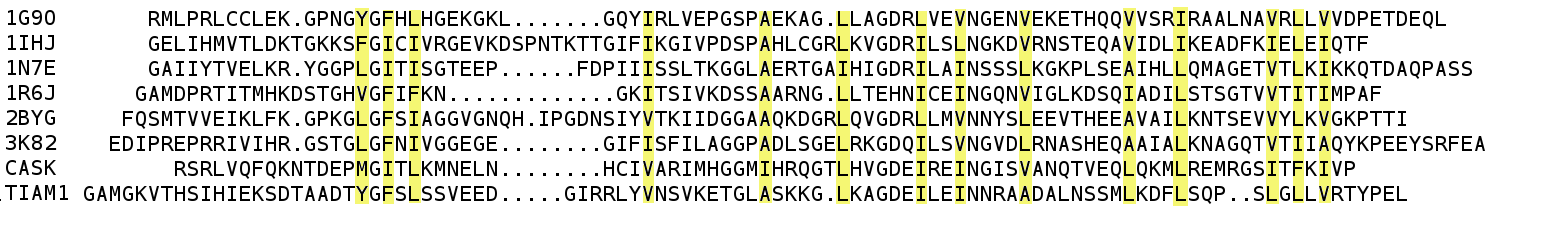
\includegraphics[width=18cm]{images/natives_alignees.png} \\
     \end{tabular}
     }
     \caption{l'aligenement des séquences natives;le cœur PDZ sélectionné est en jaune.}
\label{graph:corePDZ}
   \end{figure}


   \begin{figure}[t]
     \centering
     \begin{tabular}{c}
       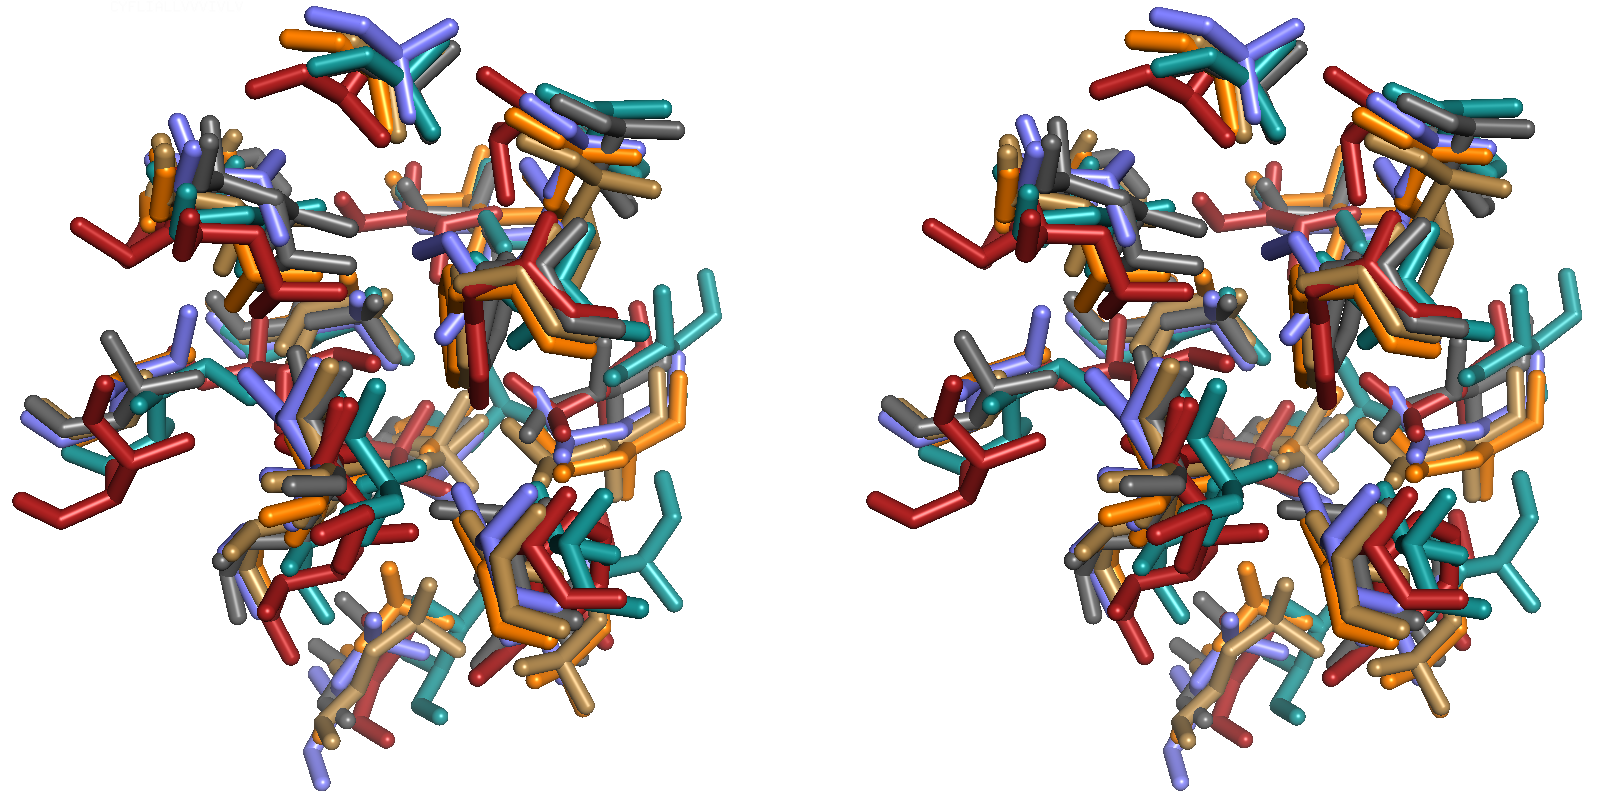
\includegraphics[width=14cm]{images/corePDZ.png} \\
     \end{tabular}
     \caption{le cœur PDZ sélectionné}
\label{graph:corePDZ}
   \end{figure}
    \begin{table}[!htbp]
      \centering

     \caption{Alignement PDZ positions du cœur}   
     \scalebox{0.5}{
       \begin{tabular}{ccccccccccccccc}
         
         \toprule
         
         \cmidrule{1-15}
         
          
         1G9O & Y & F & L & I & A & L & L & V & V & V & I & V & L & V \\
         & 24 & 26 & 28 & 39 & 48 & 53 & 59 & 62 & 67 & 75 & 79 & 86 & 88 & 90 \\ 
         1IHJ & F & I & I & I & A & L & I & L & V & V & I & I & L & I \\ 
         & 28 & 30 & 32 & 50 & 59 & 65 & 71 & 74 & 79 & 87 & 91 & 98 & 100 & 102 \\ 
         1N7E & L & I & I & I & A & I & I & I & L & A & L & V & L & I \\
         & 682 & 684 & 686 & 698 & 707 & 713 & 719 & 722 & 727 & 735 & 739 & 746 & 748 & 750 \\ 
         1R6J & V & F & F & I & A & L & I & I & V & I & L & V & I & I \\ 
         & 209 & 211 & 213 & 218 & 227 & 232 & 238 & 241 & 246 & 254 & 258 & 265 & 267 & 269 \\ 
         2BYG & L & F & I & V & A & L & L & V & L & A & L & V & L & V \\ 
         & 203 & 205 & 207 & 224 & 233 & 239 & 245 & 248 & 253 & 261 & 265 & 272 & 274 & 276 \\ 
         3K82 & L & F & I & I & A & L & I & V & L & A & L & V & I & A \\ 
         & 323 & 325 & 327 & 338 & 347 & 353 & 359 & 362 & 367 & 375 & 379 & 386 & 388 & 390 \\ 
         CASK & M & I & L & V & I & L & I & I & V & L & L & I & F & I \\ 
         & 501 & 503 & 505 & 515 & 524 & 530 & 536 & 539 & 544 & 552 & 556 & 563 & 565 & 567 \\ 
         Tiam1 & Y & F & L & V & A & L & I & I & A & L & L & L & L & V \\ 
         & 858 & 860 & 862 & 875 & 884 & 889 & 895 & 898 & 903 & 911 & 915 & 920 & 922 & 924 \\
         
         \bottomrule
         
         
         
       \end{tabular}
       }
       \label{tab:corePDZ}      
    \end{table}


    \clearpage


    
\paragraph{}

Pour réaliser les calculs Monte Carlo, les structures ont été préparés et les matrices d' énergie calculées à l'aide d'une procédure décrites précédement \cite{Schmidt09,Schmidt10}.Deux ségments manquants dans le domaine Tiam1 (résidus 851-854 et 868-869) ont été construits en utilisant le programme Modeller (51). Le ligand peptidique a été retiré de la structure PDB avant de calculer la matrice d'énergie.Pour chaque paire d'acide aminés, l'énergie d'interaction a été obtenue après 15 pas de minimisation de l'énergie, avec le backbone fixé et seulement les interactions de la paire entre les autres chaînes et le backbone. Cette courte minimisation simplifie l 'approximation discret. Les rotamères de chaînes latérales utilisés sont une version légérement étendue de la librairie de Tuffery et col \cite{Tuffery91}, qui poséde un total de 254 rotamères (sur l'ensemble des types d'acides aminés).Cette extension comprends des orientations d'hydrogème supplémentaires pour les groupes OH et SH \cite{Gaillard14}. Cette bibliothèque de rotamères a été choisié pour sa simplicité et parce qu'elle a donné de très bonnes performances dans les tests de placement de chaînes en comparaison au programme spécialisé scwlr4 qui utilise une bibliothèque beaucoup plus grande \cite{Krivov09,Gaillard16}.



\clearpage

   \begin{figure}[t]
     \centering
     \begin{tabular}{c}
       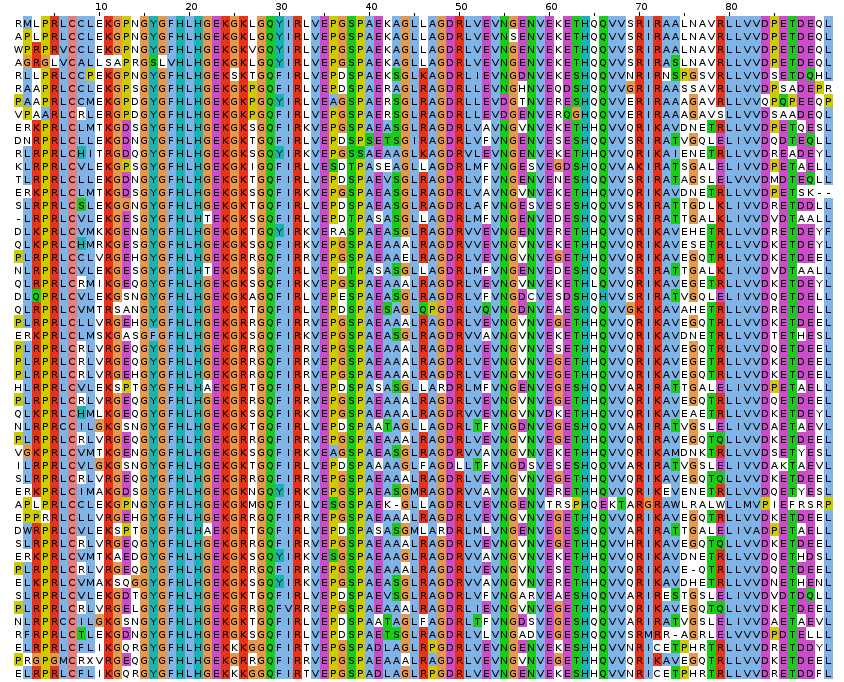
\includegraphics[width=17cm]{homologues/1G9O.png} \\
     \end{tabular}
     \caption{L'aligmenent de notre sélection de séquences homologues à la protéine NHREF (code PDB:1G9O)}
\label{align_homo:1G9O}
   \end{figure}

   \begin{figure}[t]
     \centering
     \begin{tabular}{c}
       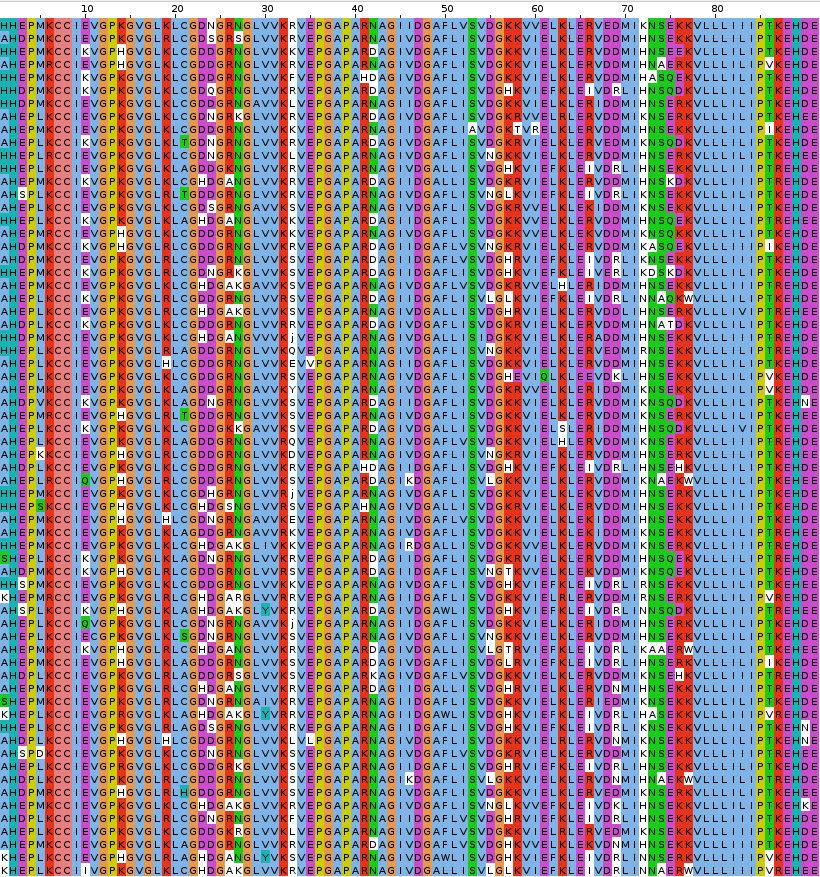
\includegraphics[width=17cm]{proteus/1G9O.png} \\
     \end{tabular}
       \caption{Une sélection de séquences proteus, parmi les 10000 séquences de meilleure énergie, obtenues avec le backbone de la protéine NHREF (code PDB:1G9O), modèle FDB}
\label{align_proteus:1G9O}
   \end{figure}

\clearpage

   \begin{figure}[t]
     \centering
     \begin{tabular}{c}
       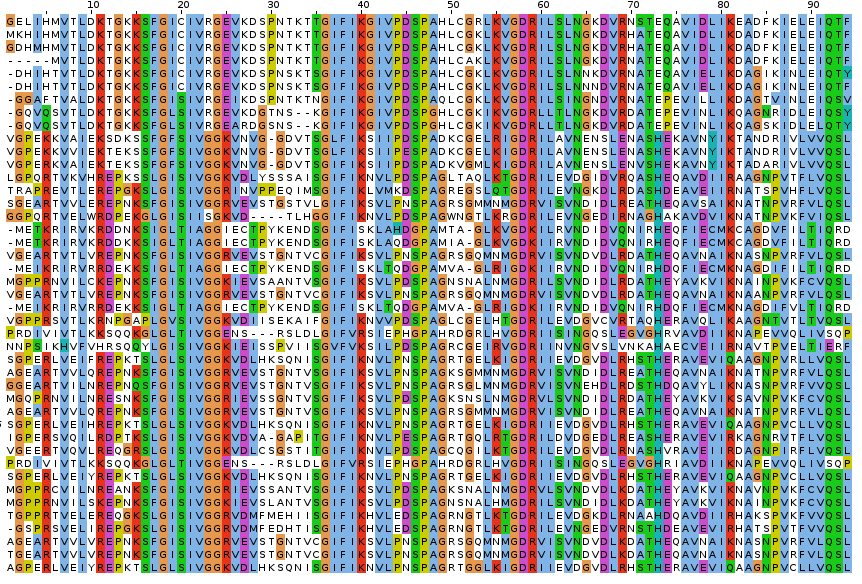
\includegraphics[width=17cm]{homologues/1IHJ.png} \\
     \end{tabular}
     \caption{L'aligmenent de notre sélection de séquences homologues à la protéine INAD (code PDB:1IHJ )}
\label{align_homo:1IHJ}
   \end{figure}

   \begin{figure}[t]
     \centering
     \begin{tabular}{c}
       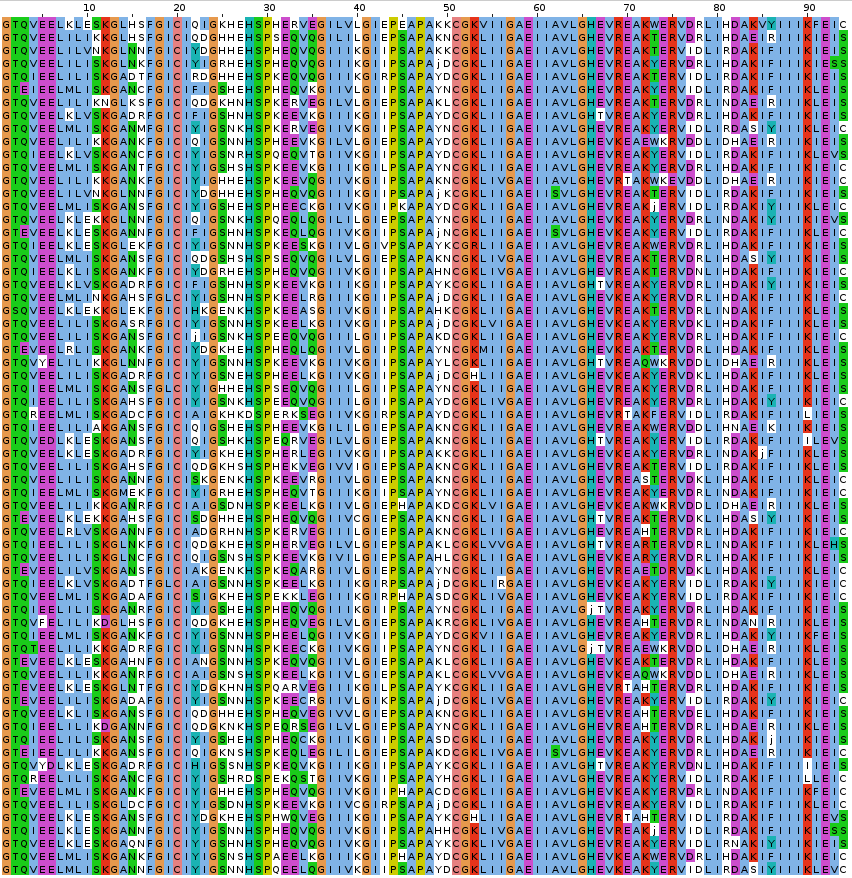
\includegraphics[width=17cm]{proteus/1IHJ.png} \\
     \end{tabular}
       \caption{Une sélection de séquences proteus, parmi les 10000 séquences de meilleure énergie, obtenues avec le backbone de la protéine INAD (code PDB:1IHJ), modèle NEA}
\label{align_proteus:1IHJ}
   \end{figure}
\clearpage

   \begin{figure}[t]
     \centering
     \begin{tabular}{c}
       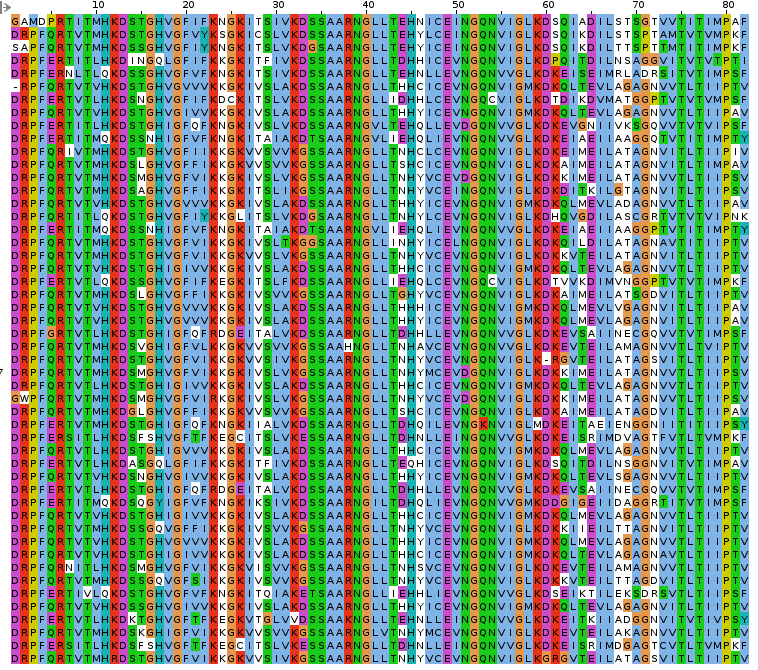
\includegraphics[width=17cm]{homologues/1R6J.png} \\
     \end{tabular}
     \caption{L'aligmenent de notre sélection de séquences homologues à la protéine Syntenin (code PDB 1R6J)}
\label{align_homo:1R6J}
   \end{figure}

   \begin{figure}[t]
     \centering
     \begin{tabular}{c}
       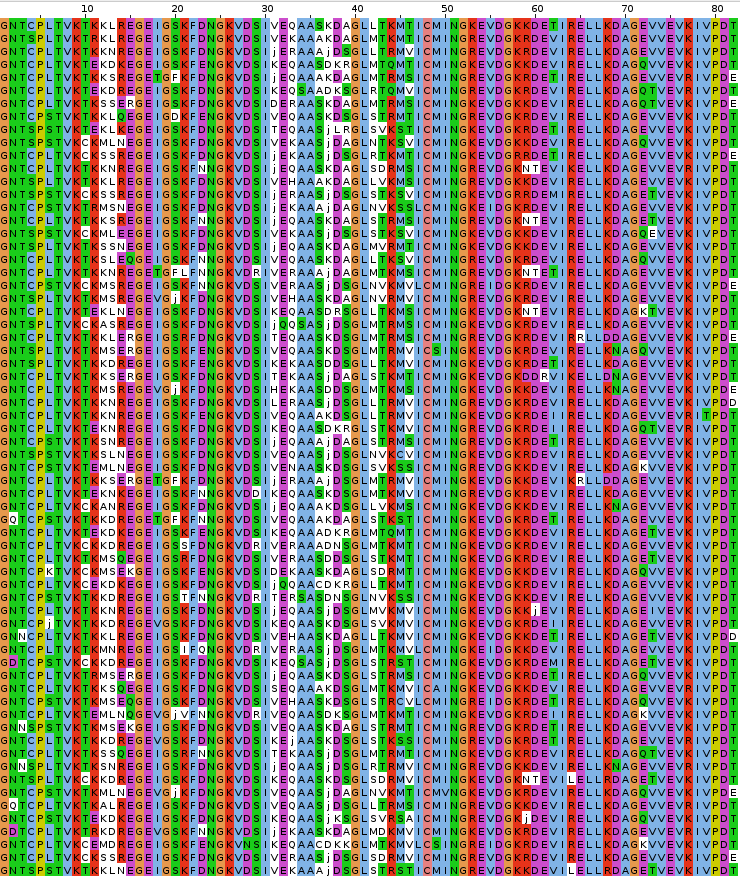
\includegraphics[width=17cm]{proteus/1R6J.png} \\
     \end{tabular}
       \caption{Une sélection de séquences proteus, parmi les 10000 séquences de meilleure énergie, obtenues avec le backbone de la protéine Syntenin (code PDB:1R6J), modèle FDB}
\label{align_proteus:1R6J}
   \end{figure}
\clearpage

   \begin{figure}[t]
     \centering
     \begin{tabular}{c}
       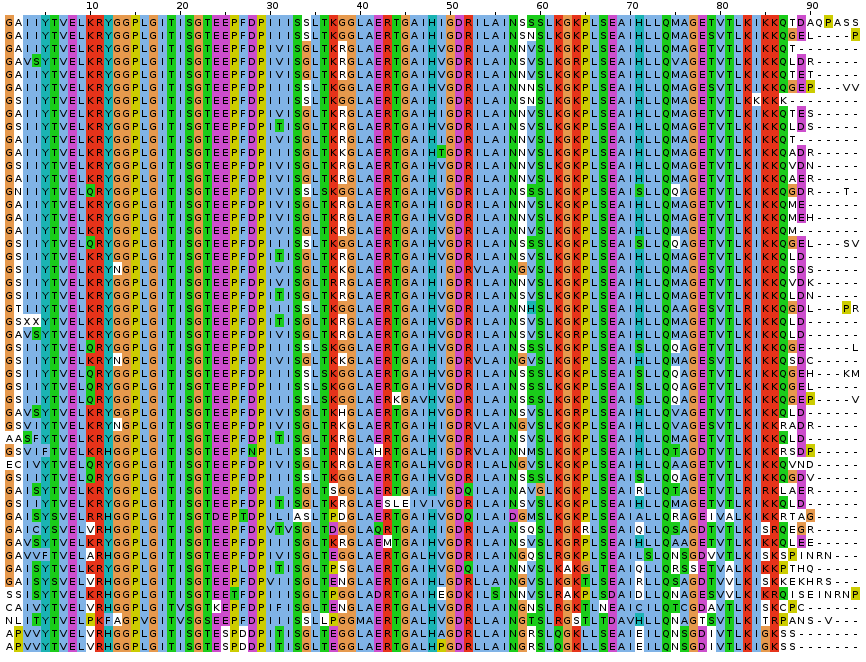
\includegraphics[width=17cm]{homologues/1N7E.png} \\
     \end{tabular}
     \caption{L'aligmenent de notre sélection de séquences homologues à la protéine GRIP (code PDB: 1N7E)}
\label{align_homo:1N7E}
   \end{figure}

   \begin{figure}[t]
     \centering
     \begin{tabular}{c}
       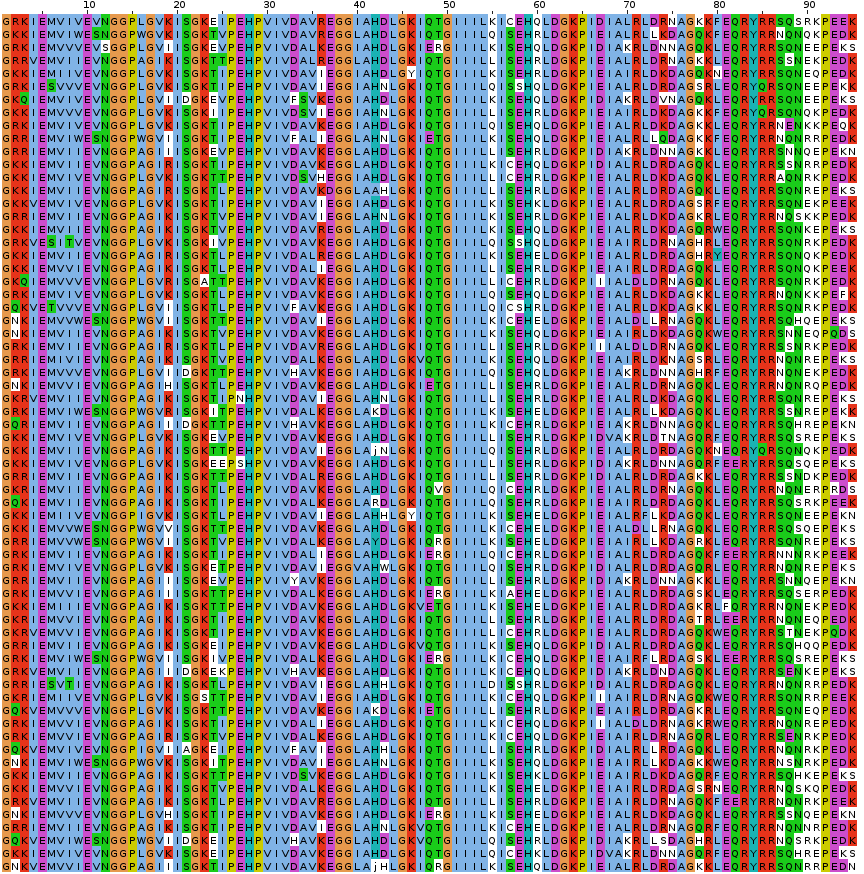
\includegraphics[width=17cm]{proteus/1N7E.png} \\
     \end{tabular}
       \caption{Une sélection de séquences proteus, parmi les 10000 séquences de meilleure énergie, obtenues avec le backbone de la protéine GRIP (code PDB:1N7E), modèle NEA}
\label{align_proteus:1N7E}
   \end{figure}
\clearpage

   \begin{figure}[t]
     \centering
     \begin{tabular}{c}
       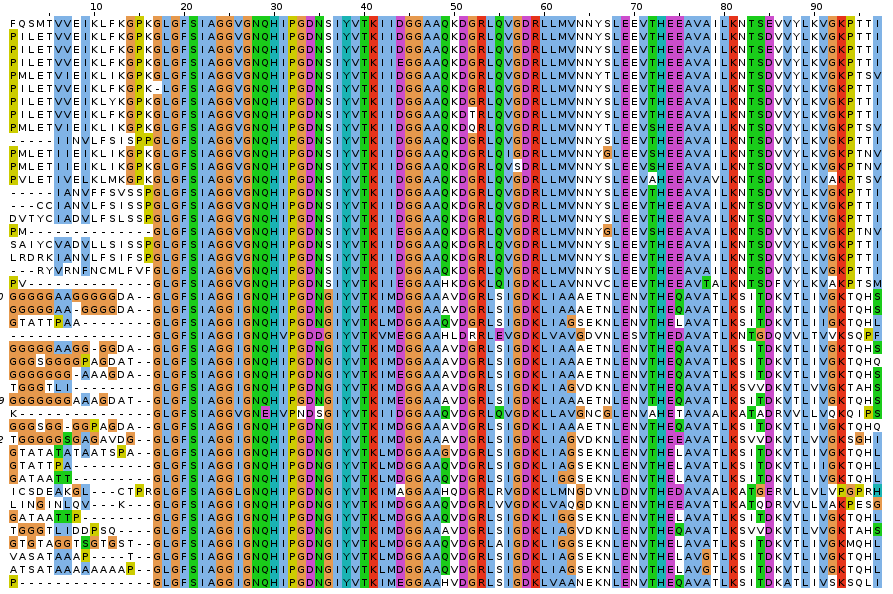
\includegraphics[width=17cm]{homologues/2BYG.png} \\
     \end{tabular}
     \caption{L'aligmenent de notre sélection de séquences homologues à la protéine DLG2 (code PDB 2BYG)}
\label{align_homo:2BYG}
   \end{figure}

   \begin{figure}[t]
     \centering
     \begin{tabular}{c}
       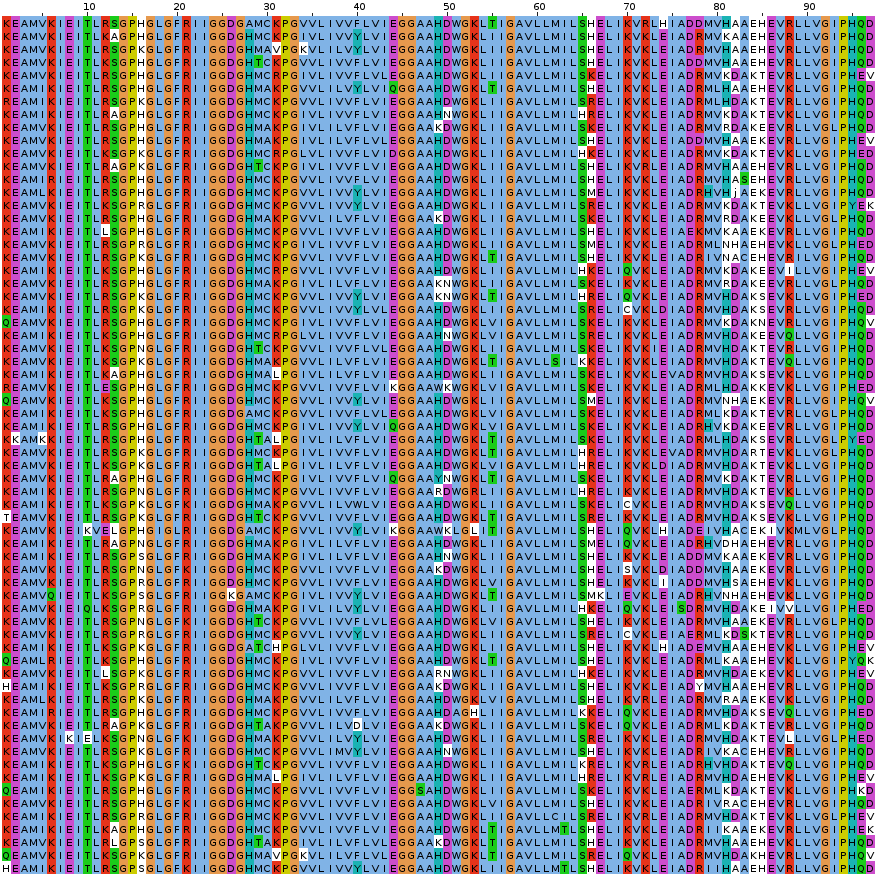
\includegraphics[width=17cm]{proteus/2BYG.png} \\
     \end{tabular}
       \caption{Une sélection de séquences proteus, parmi les 10000 séquences de meilleure énergie, obtenues avec le backbone de la protéine DLG2 (code PDB 2BYG), modèle FDB}
\label{align_proteus:2BYG}
   \end{figure}
\clearpage

   \begin{figure}[t]
     \centering
     \begin{tabular}{c}
       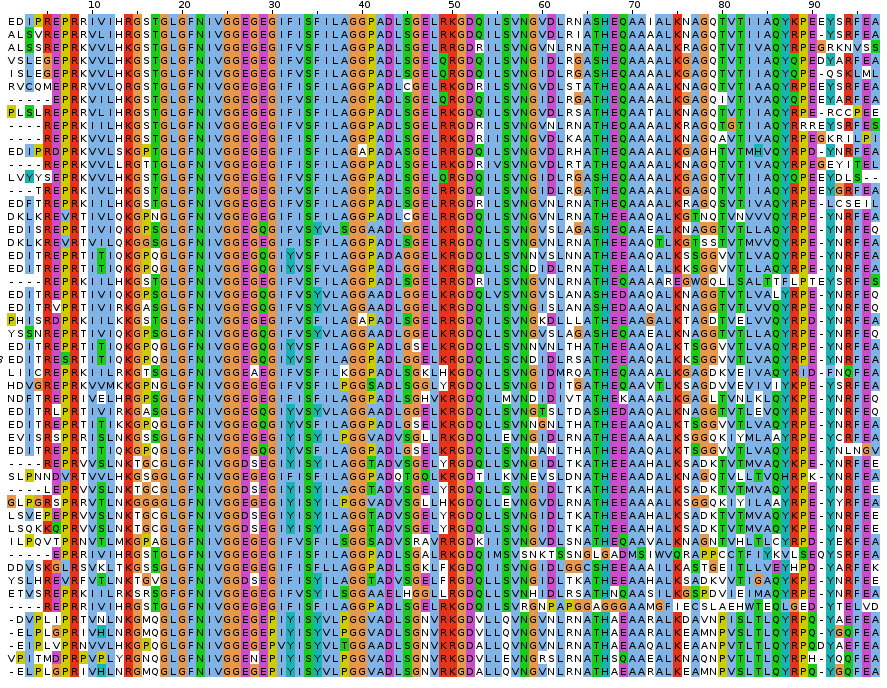
\includegraphics[width=17cm]{homologues/3K82.png} \\
     \end{tabular}
     \caption{L'aligmenent de notre sélection de séquences homologues à la protéine PSD95 (code PDB 3K82)}
\label{align_homo:3K82}
   \end{figure}

   \begin{figure}[t]
     \centering
     \begin{tabular}{c}
       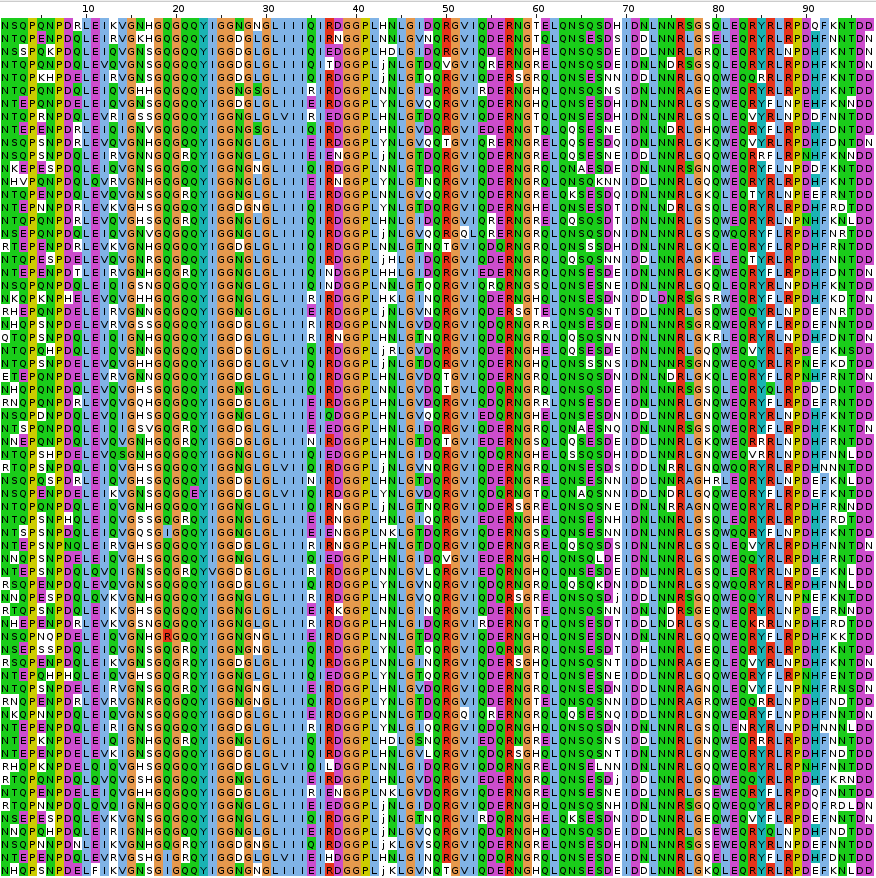
\includegraphics[width=17cm]{proteus/3K82.png} \\
     \end{tabular}
       \caption{Une sélection de séquences proteus, parmi les 10000 séquences de meilleure énergie, obtenues avec le backbone de la protéine PSD95 (code PDB:3K82), modèle FDB}
\label{align_proteus:3K82}
   \end{figure}
\clearpage

%   \begin{figure}[t]
%     \centering
%     \begin{tabular}{c}
%       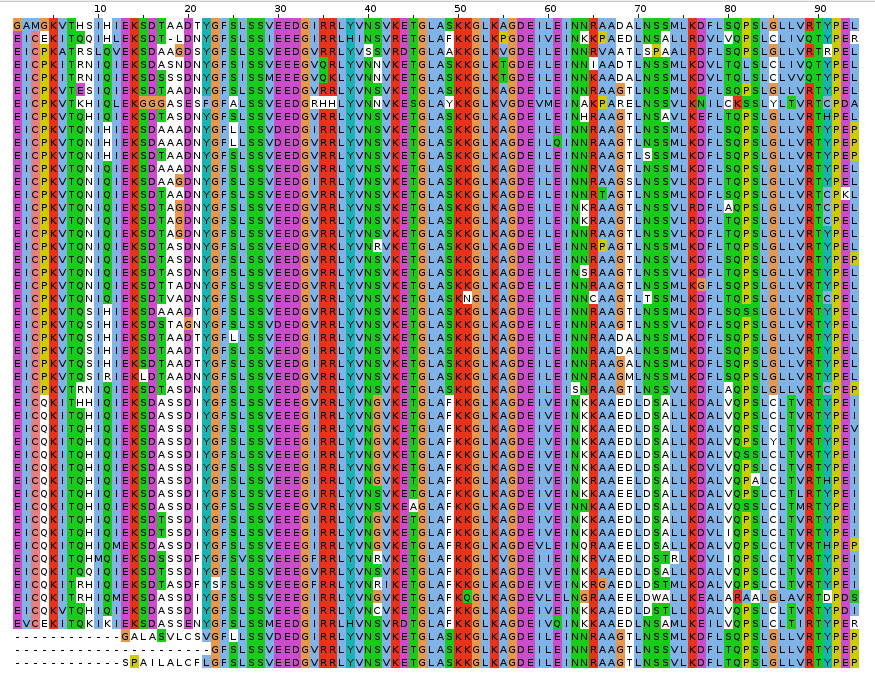
\includegraphics[width=17cm]{homologues/TIAM1.png} \\
%     \end{tabular}
%     \caption{L'aligmenent de notre sélection de séquences homologues à la protéine Tiam1 (code PDB )}
%\label{align_homo:Tiam1}
%   \end{figure}
%   
%   \begin{figure}[t]
%     \centering
%     \begin{tabular}{c}
%       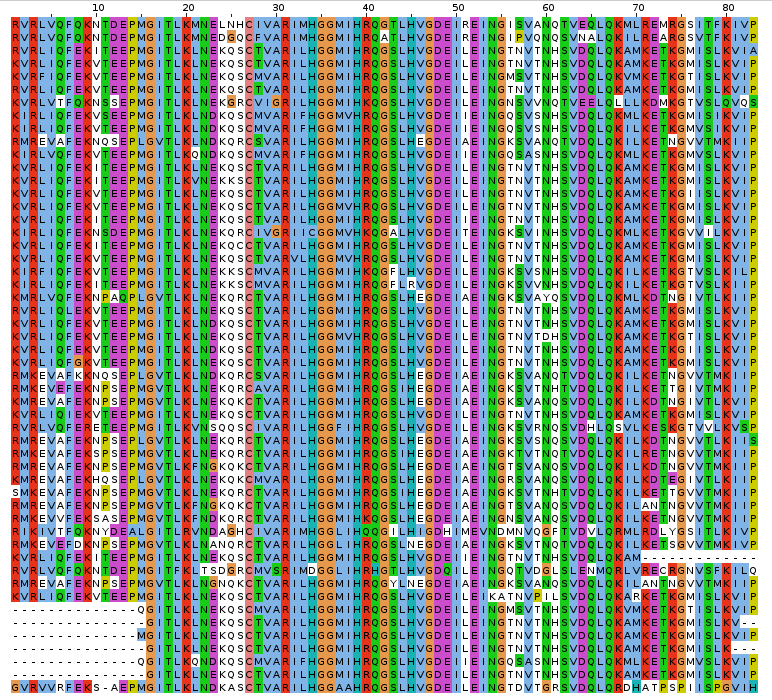
\includegraphics[width=17cm]{homologues/CASK.png} \\
%     \end{tabular}
%     \caption{L'aligmenent de notre sélection de séquences homologues à la protéine Cask (code PDB)}
%   \label{align_homo:CASK}
%   \end{figure}
%   
%\clearpage
%
    
\subsection{simulation Monte Carlo}    

La conception des séquence est réalisé avec Proteus \cite{Simonson13b}.Dans un premier temps, nous faisons des simulations où environ la moitié des position peuvent muter à la fois, pour optimiser les énergies de référence.
Ensuite,les modèles optimisé ont été testés avec des simulations où tous les positions sauf celles nativement en Gly ou Pro, sont libre de muter.
Dans les deux cas des mutations sont produites au hasard, soumises uniquement à la fonction d'énergie MMGBSA qui entraîne la simulation. Les simulations Monte Carlo utilisent des mouvements à une ou deux positions,où les rotamères,les types d'acides aminés ou les deux peuvent changer.Pour les mouvements à deux positions, la deuxième position est choisie parmi celles qui avaient une énergie d'interaction significative avec la première pour au moins une conformation du couple formé de leur chaîne latérale(c'est à dire 10 kcal/mol ou plus). De plus, l'échantillonnage est amélioré par l'échange de réplique (REMC), où plusieurs simulations MC sont exécutées en parallèle, à différenres températures. Des échanges périodiques sont effectuées comme indiquées dans \ref{para:REMC}.


\subsection{Génération de séquence Rosetta}

Des simulations Monte Carlo ont également été réalisées à l'aide du programme et de la fonction d'énergie Rosetta \cite{Baker06b}.Les simulations sont faites en utilisant la version 2015.38.58158 de la suite ( librement disponible en ligne ), en utilisant la commande:

\begin{verbatim}
fixbb -s Tiam1.pdb -resfile Tiam1.res -nstruct 10000 -ex1 -ex2 -linmem_ig 10
\end{verbatim} \normalsize


où les options ex1 et ex2 activent une recherche améliorée des rotamères pour les chaînes latérales enfouis. La dernière option correspond au calcul de l'énergie à la volée, et les paramètres par défaut sont utilisées pour les autres options.
Les résidus Gly et Pro présents dans la protéine sauvage ne sont pas autorisé à muter, et les positions qui mutent ne peuvent pas le faire en Gly  ou Pro (comme  dans les simulations Proteus).Des simulations sont exécutées pour chaque domaine PDZ jusqu'à obtenir  10 000 séquences uniques de faible énergie, ce qui correspond à des durées d'éxecution d'environ 5 minutes par séquence sur un seul coeur d'un processeur Intel récent, pour un total de 10 heures par protéines en utilisant 80 coeurs.C'est tout à fait comparable au coût des calculs Proteus , en comptant le temps de caluls de la matrice d'énergie plus celui des simulations Monte Carlo.


\subsection{Caractérisation de la séquence}

Les séquences calculées sont comparées à l'alignement Pfam pour la famille PDZ, en utilisant a matrice Blosum40 et une pénalité d'écart de -6;Cette matrice est approproée pour comparer des homologies éloignés (séquences CPD et Pfam ici). Chaque séquence Pfam est également comparée à l'aligmement Pfam, ce qui permet de comparer des séquences calculées et un couple de domaine PDZ naturels. Pour ces comparaisons Pfam/Pfam, si un domaine de test T fait partie de l'aligmenent , la comparaison T/T n'est pas prise en compte, pour être plus cohérent avec les comparaisons calculées/Pfam.L'alignement Pfam utilisée est "RP55" , composée de 12255 séquences. Les similitudes sont calculées pour d'abord les 14 résidus du coeur et pour 16 résidus de surface définis par leur presque total enfuissemebt ou exposition (voir ??)  et enfin pour l'ensemble des positions de la protéine.
Les séquences calculées sont soumises à la bibliothèque de modèle de Markov Caché Superfamily \cite{Gough01,Wilson07}  qui tente de classer les séquences selon la base de donnée structurelle de protéines SCOP \cite{Andreeva04}. La classification étant basée sur la version 1.75 de SCOP et 3.5 des Superfamily(voir plu haut).Le programme hmmscan est exécuté avec un seuil de valeur E de $10^{-10}$ et un total de 15 438 modèles dans la base SCOP. 

Pour comparer la diversité des séquences produites avec la diversité des séquences naturelles, nous utilisons l'entropie par position \cite{DurbinBK}, à partir de la formule:

\begin{equation} \label{eq:entropy}
  S_i = - \sum_{j=1}^6 f_j(i)lnf_j(i)
\end{equation} 


avec $f_j(i)$ la fréquence du type de résidu $j$ à la position $i$, Au lieu de distingué les 20 types d'acide aminé, nous utilisons six classes de résidus, correspondant à  aux groupes suivants: \{LVIMC\}, \{FYW\}, \{G\}, \{ASTP\}, \{EDNQ\} et \{KRH\}. Cette classification est a été obtenu par une analyste de cluster  sur la matrice BLOSUM 62 \label{eq:entropy} et une analyse  des énergies de contact entre résidus dans les protéines \cite{Launay07} . Pour obtenir une mesure du nombre de types d'acide aminé apparaissant à une position, on utilise l'exponentielle de l'entropie des résidus $\exp(S)$ ( qui varie de 1 à 6 ), moyenner sur l'ensemble des résidus de la chaîne protéique.


\section {Résultats}

\subsection{Structures et séquences expérimentales}


Les structures tridimensionnelles (3D) des quatre domaines PDZ de test sont représentées sur la Fig. 1A.
Quatorze résidus de noyau (identifiés visuellement) des différentes structures se superposent bien.
Tandis que les boucles et les chaînes terminales affichent de grands écarts. L'hélice $\alpha_2$ de Tiam1 est tournée légèrement vers l'extérieur par rapport aux trois autres structures (70). La figure 1b illustre la similarité structurale entre les paires de domaines PDZ. Cette similarité est déterminée par l'écart de rms (root mean square) entre  les atomes $C\alpha$ alignés structurellement et par ailleurs les identités des paires de séquences. Les écarts se situent entre $1,0$ et $2,1 \AA$  des identités de séquences entre 17 et 33 \%.La paire Tiam1/Cask on observe une identité de séquence de 33\% et et leur écart structurel de $1,7 \AA$ calculé sur 42 carbones. Les structures de syntenine et GLG2 sont plus similaires, avec une déviation structurale de $1,0 \AA$ calculé sur 60 C $\alpha$ alignés.

La conservation des séquences dans les quatre domaines PDZ et un sous-ensemble de l'alignent "seed" de Pfam est représenté sur la figure 2. Les 14 positions utilisées pour définir le noyau hydrophobe sont bien conservé conservé dans l'alignement des "seed" de Pfam, mais pas totalement. L'Arg, Lys et Gln apparaissent à certaines positions, puisque dans de petites protéines comme des domaines PDZ, Le longue partie hydrophobe  de ces chaînes latérales peut être enfui dans le noyau tout en permettant à la pointe polaire de la chaîne d'être exposé au solvant. Quelques résidus  Asp et Glu apparaissent aussi, dans les endroits où l'alignement des séquences peut ne pas très bien refléter la superposition 3D les chaînes latérales. 

\subsection{optimisation du modèle de l'état déplié}


Nous optimisons les énergies de référence $E_t^r$ pour les six protéines, en utilisant  leurs homologues naturels pour définir les fréquences d'acides aminés cibles. La constante diélectrique de la protéine P est 8. Les $E_t^r$ ont tous convergé  à 0,05 Kcal/mol près après environ 20 itérations pour la plupart des types d'acide aminés, et à 0,1 kcal/mol for les autres (ceux qui sont naturellement faiblement peuplés ) , en utilisant soit la méthode linéaire soit la méthode parabolique (équation 11 ou 12). Le tableau 2 indique les énergies de référence finales. Les valeurs $E_t^r$ ont été comparées à, et validé qualitativement avec les énergies calculées à partir d'une structure peptidique étendue, qui fournit un modèle moins empirique de l'état déplié.

\begin{table}

\scalebox{0.75}{
%%\caption{Amino acid composition (\%) from experimental and theoritical sequences after optimization. Difference between experimental and theoritical sequence are indicated into brackets.}
\begin{tabular}{lcccc|cccc|cccc|cccc}
\hline
 & \multicolumn{4}{c}{Experimental n=6}& \multicolumn{4}{c}{Model A}& \multicolumn{4}{c}{Experimental n=2}& \multicolumn{4}{c}{Model B}\\
Res & \multicolumn{2}{c}{Buried} & \multicolumn{2}{c}{Exposed} & \multicolumn{2}{c}{Buried} & \multicolumn{2}{c}{Exposed} & \multicolumn{2}{c}{Buried} & \multicolumn{2}{c}{Exposed} & \multicolumn{2}{c}{Buried} & \multicolumn{2}{c}{Exposed}\\
\hline
ALA&10.9&\multirow{3}{*}{16.9}&4.6&\multirow{3}{*}{13.4}&11.1&\multirow{2}{*}{17.0}&4.4&\multirow{2}{*}{12.0}&5.9&\multirow{3}{*}{11.2}&4.6&\multirow{3}{*}{13.4}&4.1&\multirow{2}{*}{12.7}&7.2&\multirow{2}{*}{13.6}\\
CYS&1.3&&0.5&&0.0&\multirow{2}{*}{(0.1)}&0.3&\multirow{2}{*}{(-1.4)}&1.5&&1.2&&8.6&\multirow{2}{*}{(1.5)}&5.8&\multirow{2}{*}{(0.2)}\\
THR&4.7&&8.3&&5.9&&7.3&&3.8&&7.6&&0.0&&0.6&\\
\hline
ASP&4.3&\multirow{2}{*}{6.8}&6.0&\multirow{2}{*}{17.9}&4.5&\multirow{1}{*}{6.7}&5.6&\multirow{1}{*}{16.7}&3.5&\multirow{2}{*}{9.6}&6.2&\multirow{2}{*}{16.7}&7.4&\multirow{1}{*}{9.4}&8.0&\multirow{1}{*}{16.1}\\
GLU&2.5&&11.9&&2.2&(-0.1)&11.1&(-1.2)&6.1&&10.5&&2.0&(-0.2)&8.1&(-0.6)\\
\hline                          
ASN&2.6&\multirow{2}{*}{4.7}&6.7&\multirow{2}{*}{12.2}&2.5&\multirow{1}{*}{4.7}&7.5&\multirow{1}{*}{14.0}&1.9&\multirow{2}{*}{2.7}&7.4&\multirow{2}{*}{16.1}&1.8&\multirow{1}{*}{2.8}&8.6&\multirow{1}{*}{17.1}\\
GLN&2.1&&5.5&&2.2&(0.0)&6.5&(1.8)&0.8&&8.7&&1.0&(0.1)&8.5&(1.0)\\
\hline                                                                                       
HIP&1.2&\multirow{3}{*}{1.2}&5.0&\multirow{3}{*}{5.0}&1.0&\multirow{2}{*}{1.1}&5.2&\multirow{2}{*}{5.6}&0.7&\multirow{3}{*}{0.7}&4.7&\multirow{3}{*}{4.7}&0.1&\multirow{2}{*}{0.9}&1.8&\multirow{2}{*}{4.5}\\
HIE&0.0&&0.0&&0.1&\multirow{2}{*}{(-0.1)}&0.4&\multirow{2}{*}{(0.6)}&0.0&&0.0&&0.6&\multirow{2}{*}{(0.2)}&2.2&\multirow{2}{*}{(-0.2)}\\
HID&0.0&&0.0&&0.0&&0.0&&0.0&&0.0&&0.2&&0.5&\\
\hline                                                                                  
ILE&16.0&\multirow{3}{*}{50.7}&4.2&\multirow{3}{*}{14.0}&16.9&\multirow{2}{*}{52.1}&4.1&\multirow{2}{*}{14.0}&15.7&\multirow{3}{*}{49.6}&4.1&\multirow{3}{*}{14.4}&25.1&\multirow{2}{*}{46.7}&8.4&\multirow{2}{*}{15.3}\\
VAL&16.5&&5.4&&16.7&\multirow{2}{*}{(1.4)}&5.6&\multirow{2}{*}{(0.0)}&13.5&&5.5&&12.8&\multirow{2}{*}{(-2.9)}&3.3&\multirow{2}{*}{(0.9)}\\
LEU&18.2&&4.4&&18.5&&4.3&&20.4&&4.8&&8.8&&3.6&\\
\hline                                                                              
\multirow{2}{*}{LYS}&\multirow{2}{*}{2.5}&\multirow{2}{*}{2.5}&\multirow{2}{*}{10.9}&\multirow{2}{*}{10.9}&\multirow{2}{*}{1.5}&1.5&\multirow{2}{*}{13.0}&13.0&\multirow{2}{*}{6.5}&\multirow{2}{*}{6.5}&\multirow{2}{*}{10.1}&\multirow{2}{*}{10.1}&\multirow{2}{*}{5.5}&5.5&\multirow{2}{*}{10.8}&10.8\\
&&&&&&(-1.0)&&(2.1)&&&&&&(-1.0)&&(0.7)\\
\hline                                                                        
\multirow{2}{*}{MET}&\multirow{2}{*}{0.9}&\multirow{2}{*}{0.9}&\multirow{2}{*}{1.5}&\multirow{2}{*}{1.5}&\multirow{2}{*}{1.6}&1.6&\multirow{2}{*}{1.4}&1.4&\multirow{2}{*}{5.0}&\multirow{2}{*}{5.0}&\multirow{2}{*}{1.4}&\multirow{2}{*}{1.4}&\multirow{2}{*}{5.9}&5.9&\multirow{2}{*}{1.4}&1.4\\
&&&&&&(0.7)&&(-0.1)&&&&&&(0.9)&&(0.0)\\
\hline                                                                         
\multirow{2}{*}{ARG}&\multirow{2}{*}{2.8}&\multirow{2}{*}{2.8}&\multirow{2}{*}{8.7}&\multirow{2}{*}{8.7}&\multirow{2}{*}{2.5}&2.5&\multirow{2}{*}{6.1}&6.1&\multirow{2}{*}{1.8}&\multirow{2}{*}{1.8}&\multirow{2}{*}{9.5}&\multirow{2}{*}{9.5}&\multirow{2}{*}{2.2}&2.2&\multirow{2}{*}{9.1}&9.1\\
&&&&&&(-0.3)&&(-2.6)&&&&&&(0.4)&&(-0.4)\\
\hline                                                                                  
\multirow{2}{*}{SER} &\multirow{2}{*}{5.3}&\multirow{2}{*}{5.3}&\multirow{2}{*}{7.6}&\multirow{2}{*}{7.6}&\multirow{2}{*}{4.3}&4.3&\multirow{2}{*}{8.7}&8.7&\multirow{2}{*}{4.7}&\multirow{2}{*}{4.7}&\multirow{2}{*}{10.2}&\multirow{2}{*}{10.2}&\multirow{2}{*}{4.9}&4.9&\multirow{2}{*}{10.7}&10.7\\
&&&&&&(-1.0)&&(1.1)&&&&&&(0.2)&&(0.5)\\
\hline                                                         
PHE      &4.1&\multirow{2}{*}{4.1}&2.4&\multirow{2}{*}{2.4}&4.5&\multirow{1}{*}{4.6}&2.1&\multirow{1}{*}{2.1}&5.0&\multirow{2}{*}{5.0}&0.4&\multirow{2}{*}{0.4}&3.2&\multirow{1}{*}{5.5}&0.3&\multirow{1}{*}{0.5}\\
TRP&0.0&&0.0&&0.1&(0.5)&0.0&(-0.3)&0.0&&0.0&&2.3&(0.5)&0.2&(0.1)\\
\hline                                                                                                                                                                                   
\multirow{2}{*}{TYR}&\multirow{2}{*}{2.6}&\multirow{2}{*}{2.6}&\multirow{2}{*}{1.2}&\multirow{2}{*}{1.2}&\multirow{2}{*}{2.2}&2.2&\multirow{2}{*}{0.4}&0.4&\multirow{2}{*}{2.9}&\multirow{2}{*}{2.9}&\multirow{2}{*}{0.9}&\multirow{2}{*}{0.9}&\multirow{2}{*}{3.4}&3.4&\multirow{2}{*}{0.9}&0.9\\
&&&&&&(-0.4)&&(-0.8)&&&&&&(0.5)&&(0.0)\\
\hline                                                                                                                                                                            
GLY&0.8&\multirow{2}{*}{0.9}&3.1&\multirow{2}{*}{4.9}&0.0&\multirow{1}{*}{0.0}&0.0&\multirow{1}{*}{0.0}&0.0&\multirow{2}{*}{0.3}&1.7&\multirow{2}{*}{2.1}&0.0&\multirow{1}{*}{0.0}&0.0&\multirow{1}{*}{0.0}\\
PRO&0.1&&1.8&&0.0&(-0.9)&0.0&(-4.9)&0.3&&0.4&&0.0&(-0.3)&0.0&(-2.1)\\
\hline
\end{tabular}
}
\end{table}





Le tableau 3 compare les fréquences d'acide aminé des homologues naturels et les calculées. La population théorique des différentes classes d'acide aminé ont bien rejoint l' expérience, avec des écarts de rms d'environ 1\%, pour les positions exposées et enfuies. L'accord entre les types d'acide aminé est moins bon avec des écarts de rms de 3,9\% et 2,4\% (enfuie/exposés).La distribution des fréquences intra classe dépend par construction du $\delta E_t^r$ défini dans pour chaque classe, qui ont était calculés avec la mécanique moléculaire (voir méthodes, équation 15). Ainsi une seconde série de 20 itérations est effectué en relâchant cette contrainte alors l'optimisation ne se fait plus sur les six classes de type d'acide aminé , mais directement sur les dix-huit types possibles (les positions Pro et Gly étant fixées). 


    \begin{table}[!htbp]
      \centering

      \begin{tabular}{ccc}

        \toprule
        Type d'acides aminés & Pos. Enf. & Pos Exp. \\
        \cmidrule{1-3}

        ALA & 0.00     &  0.00     \\
        ARG & -28.29   &  -28.90   \\
        ASN & -5.94    &  -6.00    \\
        ASP & -9.19    &  -9.80    \\
        CYS & -1.04    &  -1.04    \\
        GLN & -4.72    &  -4.78    \\
        GLU & -7.90    &  -8.51    \\
        HID & 11.96    &  12.39    \\
        HIE & 11.43    &  11.85    \\
        HIP & 14.53    &  14.96    \\
        ILE & 4.72     &  2.11     \\
        LEU & 1.17     &  -1.44    \\
        LYS & -4.56    &  -4.47    \\
        MET & -2.78    &  -3.54    \\
        PHE & -0.37    &  -2.55    \\
        SER & -3.73    &  -2.80    \\
        THR & -3.82    &  -3.82    \\
        TRP & -1.61    &  -3.79    \\
        TYR & -4.20    &  -6.10    \\
        VAL & 0.83     &  -1.77    \\

        \bottomrule


      \end{tabular}      
      \caption{Les énergies de référence obtenues avec l'optimisation 6 protéines.}
\label{tab:RefEner_groupes}      
    \end{table}




\subsection{Évaluation de la qualité des séquences obtenues}

\paragraph{Tests de reconnaissance de famille}

Les simulations Proteus utilisent l'algorithme Monte-Carlo avec échange de répliques (REMC) avec huit répliques et 750 millions de pas par réplique, avec des énergies thermiques kT  qui varient de 0,125 à 3 kcal/mol. Toutes les positions sont autorisées à muter librement dans tout les types d'acides aminés excepté Gly et Pro. Les simulations ont été faites avec la fonction d'énergie MMGBSA, sans aucune introduction de biais vers  les séquences naturelles ni aucune limite sur le nombre de mutations. Les 10 000 séquences avec les énergies les plus faibles parmi celles échantillonnées par au moins une des répliques MC sont retenues pour l'analyse. De la même façon, 10 000 séquences produites par Rosetta ont était retenue. Ces séquences sont analysées par les outils de reconnaissance de repliment "Superfamily" (\ref{superfamily}) , voir tableau 4.Avec une constante diélectrique de 8, nous avons obtenu un pourcentage élevé de séquences correctement associées à la famille et superfamille PDZ: 91\% pour Tiam1 et 100\% pour Cask, avec des "E-values" d'environ $10^{-3}$ pour les affectations à la famille.Ces valeurs sont semblables à celles obtenues par Rosetta (90 et 98\% de reconnaissance de la famille pour Tiam1  et Cask).

\paragraph{Séquences et diversité de séquence}
Les séquences Tiam1 et Cask calculées par Proteus, par Rosetta et les séquences naturelles sont montrées à la figure 3. Pour les quatorze résidus du noyau et la figure 4 pour les seize résidus de surface (Tiam1  uniquement). Les séquences sont représentées par des logos de séquences. Comme on l'a vu dans de nombreuses études de CPD antérieures (30,72) l'accord avec l'expérience pour les positions du cœur est très bon, alors que l'accord en ce qui concerne les résidus de surface est nettement plus faible. La diversité des séquences naturelles et des séquences calculées est caractérisées par la moyenne sur la séquence de l'exponentielle de l'entropie résiduel (voir Méthodes), ce qui correspond à un nombre moyen de classe de séquence échantillonnées par position. Par exemple, une valeur de 2 à une position particulière indique que les acides aminés de deux des six classes sont présents à cette position au sein de l'ensemble des séquences analysées. Une valeur moyenne globale de deux indique qu'en moyenne, deux classes d'acides aminés sont présentes à n'importe quelle position dans les séquences analysées. Comme référence l'ensemble Pfam RP55 et 12 255 séquences naturelles a une entropie moyenne de 3,4.Le regroupement des séquences Tiam1 et Cask calculés  donne une entropie de 2,2 avec Rosetta et 2,0 avec Proteus. Ce qui indique que ces deux seules géométries de backbone ne peuvent pas être attendre les mêmes niveaux de diversités que le grand ensemble RP55. Prenant les 10000 séquences Monte-Carlo de meilleure énergie échantillonnées à température ambiante (au lien des 10 000 de plus basses énergies échantillonnées collectivement par toutes les répliques à toutes les températures) et la mise en commun de Tiam1 et Cask donne une entropie globale plus élevée de 2,9 avec Proteus. Pour Rosetta, l' entropie dans le noyau est seulement légèrement inférieure à la moyenne sur toutes les positions. Pour Proteus, c'est nettement inférieur (1,25). Pour les séquences Pfam-Rp55, cette entropie est de 1,8.

    \begin{table}[!htbp]
      \centering

      \begin{tabular}{ccccc}

        \toprule
        Protein & Proteus & Rosetta & Pfam seed \\
        \cmidrule{1-4}
        1G9O  & 1.38 & 1.45 & 3.15  \\
        1IHJ  & 1.37 & 1.55 & 3.06  \\
        1N7E  & 1.33 & 1.44 & 3.09  \\
        1R6J  & 1.39 & 1.43 & 3.03  \\
        2BYG  & 1.24 & 1.57 & 3.11  \\
        3K82  & 1.27 & 1.40 & 3.15  \\
        6prots & 2.42  & 2.88 &    \\
        CASK  & 1.55 & 1.68 & 3.15  \\
        TIAM1 & 1.22 & 1.57 & 3.15  \\

        \bottomrule

      \end{tabular}      
      \caption{Moyenne de l'exponentiel de l'entropie sur les ensembles des positions des protéines}
\label{tab:Entropie_PDZ}      
    \end{table}


        \begin{table}[!htbp]
      \centering

      \begin{tabular}{ccccc}

        \toprule
        Sequences & Proteus & Rosetta & Proteus (inclus G et P) & Rosetta (inclus G et P)\\
        \cmidrule{1-5}
        1G9O  & 28 &  43 & 44 & 59 \\
        1IHJ  & 26 &  40 & 35 & 49 \\
        1N7E  & 33 &  48 & 50 & 65 \\
        1R6J  & 26 &  46 & 38 & 58 \\
        2BYG  & 28 &  46 & 42 & 61 \\
        3K82  & 36 &  52 & 54 & 70 \\
        TIAM1 & 18 &  25 & 28 & 30 \\
        CASK  & 17 &  28 & 28 &  39 \\

        \bottomrule

      \end{tabular}      
      \caption{Pourcentage d'identité moyen à la séquence native}
\label{tab:Entropie_PDZ}      
    \end{table}



\begin{table}[h]
  
  \begin{tabular}{cccccc}
    
    \toprule
    Protein & Match/seq & Superfamily & Superfamily & Family & Family \\
            & size      & Evalue      & success     & Evalue & success\\
    \cmidrule{1-6}
    1G9O  & 81/91 &  2.00e-12 & 10000  & 9.97e-3 & 10000  \\
    1IHJ  & 84/94 &  4.80e-11 & 10000  & 2.83e-3 & 10000  \\
    1N7E  & 82/95 &  4.73e-8  & 10000  & 5.56e-3 & 10000  \\
    1R6J  & 63/91 &  4.01e-4  &  9999  & 1.05e-2 &  9999  \\
    2BYG  & 84/97 &  3.82e-10 & 10000  & 3.75e-3 & 10000  \\
    3K82  & 46/97 &  7.65e-1  &  5029  & 4.06e-2 &  4719  \\

    \bottomrule        
  \end{tabular}   
  \caption{Résultats Superfamily pour les séquences Proteus avec le modèle B N=6 (E ref optimisées sur 20 cycles selon les classes + 20 cycles selon les types).}   
  \label{tab:superfamily_model_B6}       
\end{table}


        
\begin{table}[h]

  \begin{tabular}{cccccc}
    
    \toprule
    Protein & Match/seq & Superfamily & Superfamily & Family & Family \\
            & size      & Evalue      & success     & Evalue & success\\
    \cmidrule{1-6}
    1G9O  & 79/91   &    1.3e-13 & 10000 & 2.2e-3 & 10000 \\
    1IHJ  & 85/94   &    7.4e-14 & 10000 & 3.7e-3 & 10000 \\
    1N7E  & 84/95   &    2.2e-10 & 10000 & 1.2e-3 & 10000 \\
    1R6J  & 76/82   &    7.3e-13 & 10000 & 1.8e-3 & 10000 \\
    2BYG  & 86/97   &    1.3e-9  & 10000 & 9.6e-4 & 10000 \\
    3K82  & 90/97   &    3.7e-23 & 10000 & 5.2e-4 & 10000 \\
    \bottomrule        
  \end{tabular}   
  \caption{Résultats Superfamily pour les séquences Rosetta des  protéines PDZ}   
  \label{tab:superfamily_bestRE}       
\end{table}

        
\paragraph{Scores de similarité Blosum}

La figure 5 montre les scores de similarité Blosum40 entre les séquences calculées et les séquences naturelles. Avec Proteus, pour Tiam1 et Cask, les similitudes globales se chevauchent au pied du somment des scores naturels, sont comparables aux valeurs des séquences Rosetta. Pour les résidus de surface, montrés séparément, la similitude avec les séquences naturelles est faible (scores inférieurs à zéro), à la fois pour Proteus et Rosetta. Avec $\epsilon_p=8$, Proteus donne presque la même similitude moyenne sur toutes les postions Tiam1 et Cask, par exemple.
Alors que les scores de similarité Proteus par rapport à Pfam  sont comparables à Rosetta (figure 5) , les scores d'identité par rapport à la séquence sauvage sont significativement plus élevés avec Rosetta. Les scores d'identité excluants (respectivement incluant) les postions Gly et Pro (qui ne sont pas mutables) sont de 20\% (28\%) pour Proteus contre 26\% (34\%) pour Rosetta.


   \begin{figure}[t]
     \centering
     \begin{tabular}{cc} 
       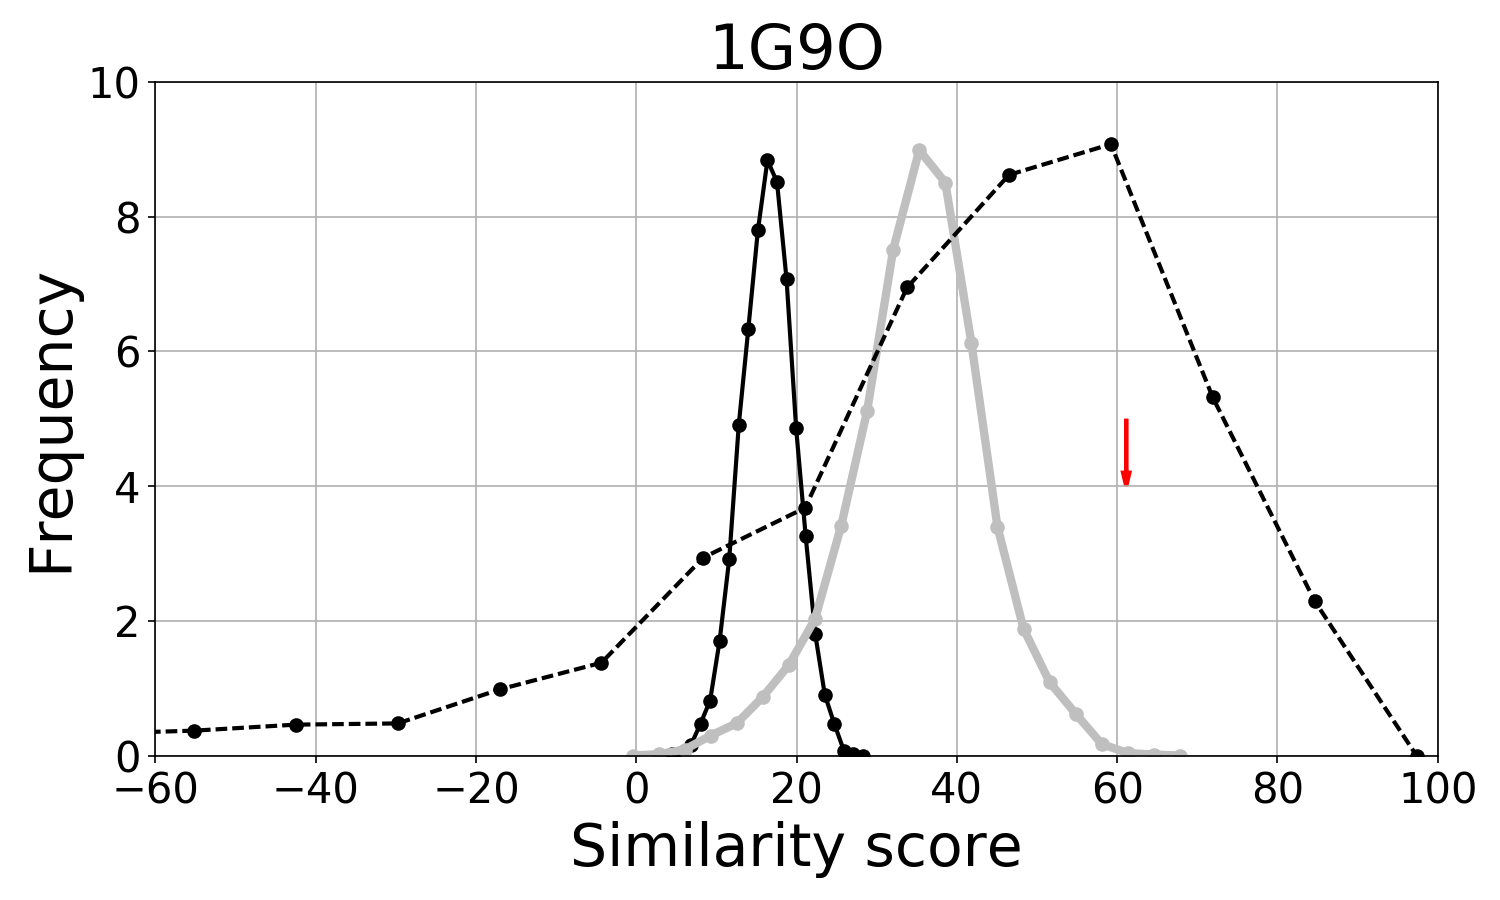
\includegraphics[width=8.4cm]{modelB6+/1G9O_simil_full.png} &
       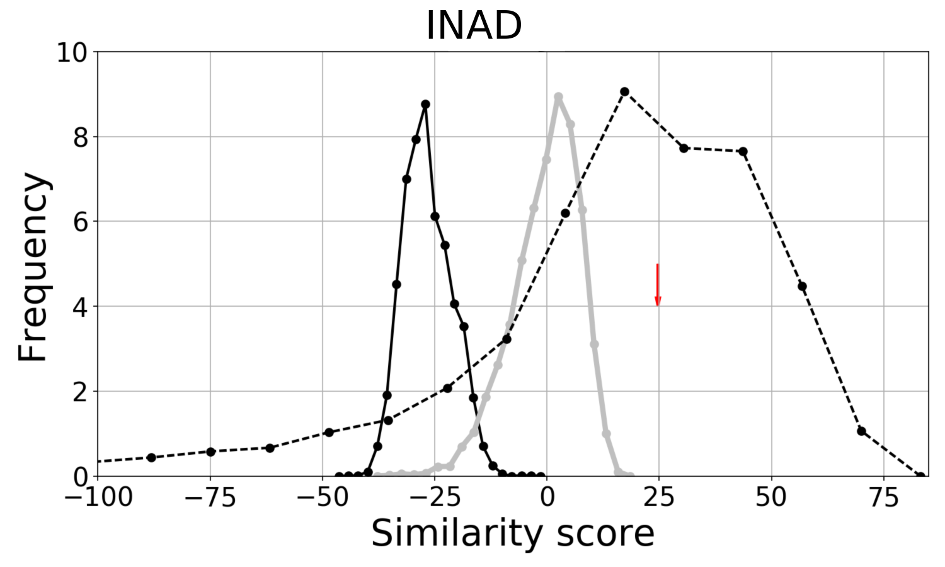
\includegraphics[width=8.4cm]{modelB6+/1IHJ_simil_full.png} \\
       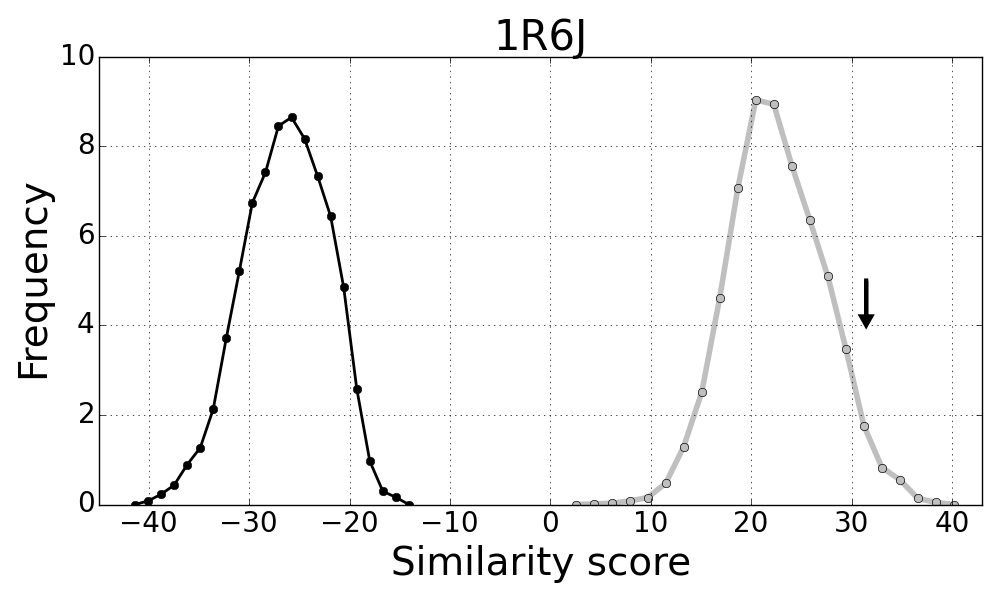
\includegraphics[width=8.4cm]{modelB6+/1R6J_simil_full.png} &
       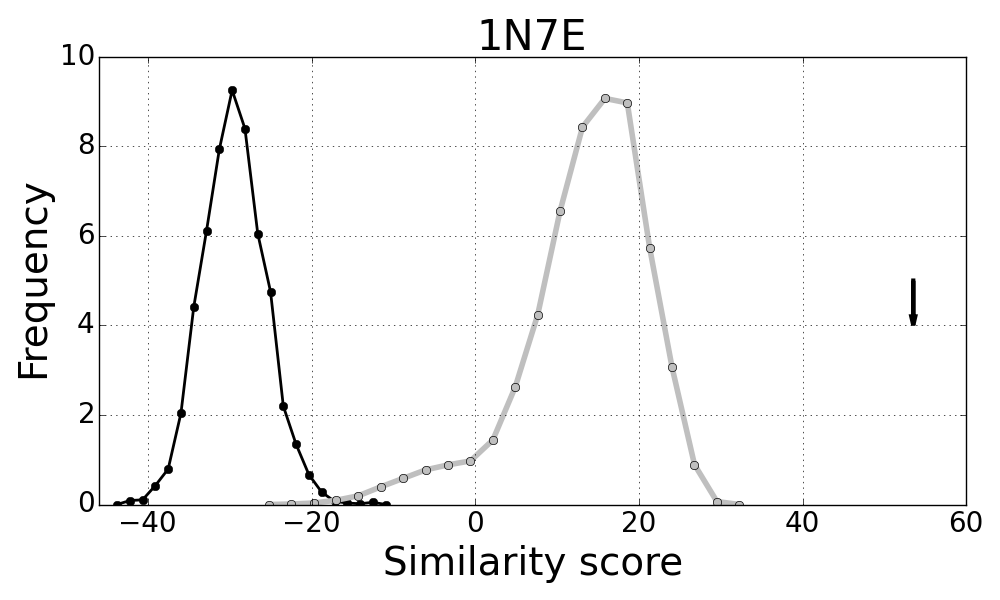
\includegraphics[width=8.4cm]{modelB6+/1N7E_simil_full.png} \\
       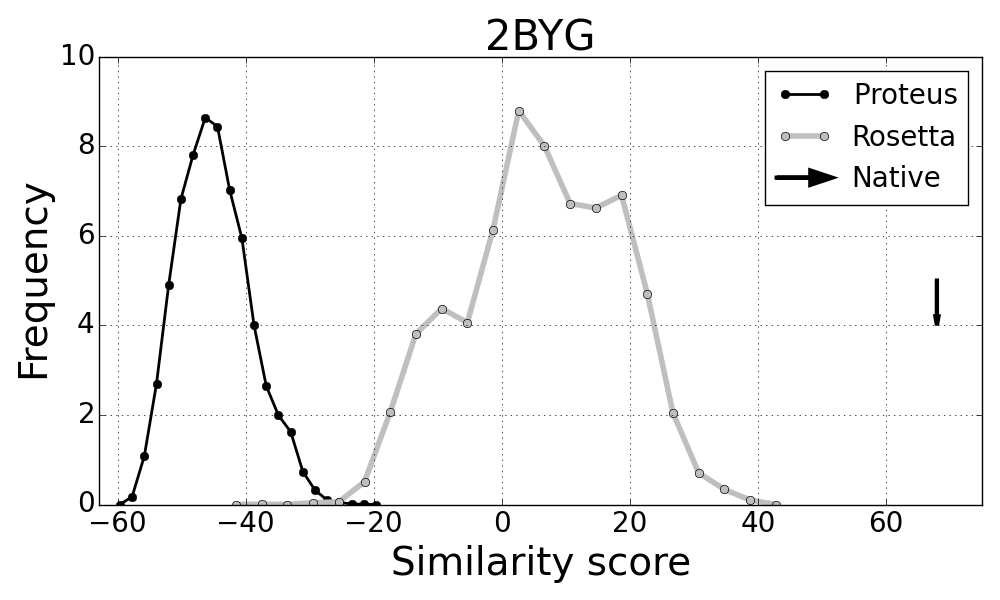
\includegraphics[width=8.4cm]{modelB6+/2BYG_simil_full.png} &
       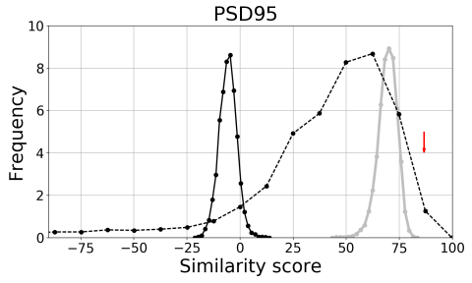
\includegraphics[width=8.4cm]{modelB6+/3K82_simil_full.png} \\
     \end{tabular}
  \caption{Similarité des séquences des 6 protéines produites par proteus modèle B N=6 (E ref optimisées sur 20 cycles selon les classes + 20 cycles selon les types) et Rosetta à l'alignement Pfam RP55, sur l'ensemble des positions.}

   \end{figure}


\paragraph{Tests de validation croisée}
Comme premier test de validation croisée,nous utilisons les énergies de référence optimisées à l'aide des homologues de Tiam1 et Cask à deux entre domaines PDZ: DLG2 et Syntenine. Les scores Superfamily sont comparables à ceux obtenus pour Tiam1 et Cask, avec 100\% de reconnaissance de la famille (tableau 4). Les séquences calculées avec Rosetta pour la DLG2 et la Syntenine ont également obtenu une reconnaissance  de la famille dans 100\% des cas. Comme validation croisée supplémentaire,nous optimisons les énergies de références en utilisant un ensemble alternatif de domaines PDZ: DLG2, Syntenin,
PSD95, GRIP, INAD et NHERF. Pour distinguer les variantes du modèle, nous nous référons à cette nouvelle variante en tant que modèle n=6 (il utilise six domaines PDZ pour la paramétrisation) et le modèle initial comme modèle n=2. Les énergies de référence  nouveau n=6,  sont alors utilisées pour produire des séquences Tiam1 et Cask , qui sont alors soumisses aux tests Superfamily et des calculs de similarité. La performance de Tiam1 sur la superfamille est légèrement dégradée par rapport au précédent modèle n=2.Le score superfamily de Tiam1 diminue de 90,6\% à 76,6\% pour la reconnaissance de la famille. Les scores de Cask sont inchangés. Les histogrammes des scores de similarité Blosum montrent que les scores globaux pour Tiam1 et Cask avec n=6 sont très semblables à ceux du modèle n=2, alors que les scores pour les positions centrales sont nettement améliorés. Pour DLG2 et Syntenine, nous calculons également les scores de similarité en utilisant à la fois le modèle n=2 et le modèle n=6. Les scores de similarité avec n=2 sont légèrement plus faibles qu'avec n=6, comme on pouvait le prévoir.Le score global a diminué d'environ 20 points pour la Synténine et environ 10 points pour DLG2. dans l'ensemble, les modèles de validation croisée ont légèrement dégradé les performances. Ainsi, pour tout domaine d'intérêt PDZ, Il est préférable d'optimiser les énergies de référence spécifiquement pour ce domaine plutôt que de transférer des valeurs paramétrées en utilisant d'autres domaines PDZ. 

\paragraph{Modèle FDB}


\begin{table}[h]
  \raggedleft{}
  
  \begin{tabular}{ccccccc}
    
    \toprule
    Model &Protein & Match/seq & Superfamily & Superfamily & Family & Family \\
            & size      & Evalue      & success     & Evalue & success\\
    \cmidrule{1-7}
    Proteus    & 1G9O  & 80/91 &  8.54 $10^{-14}$  & 10000  & 8.94 $10^{-3}$ & 10000 \\
    FDB        & 1R6J  & 70/82 &  2.85 $10^{-6}$   & 10000  & 2.69 $10^{-3}$ & 10000 \\
    epsilon=4  & 2BYG  & 88/97 &  3.26 $10^{-12}$  & 10000  & 1.96 $10^{-3}$ & 10000 \\
    \cmidrule{1-7}
    \multirow{3}{*}{Rosetta} & 1G9O  & 79/91  &  1.3 $10^{-13}$ & 10000 & 2.2 $10^{-3}$ & 10000 \\
                             & 1R6J  & 76/82  &  7.3 $10^{-13}$ & 10000 & 1.8 $10^{-3}$ & 10000 \\
                             & 2BYG  & 86/97  &  1.3 $10^{-9}$  & 10000 & 9.6 $10^{-4}$ & 10000 \\    
    \cmidrule{1-7}
    Proteus    & 1G9O  & 62/91 & 3.22 $10^{-3}$  & 9857  & 1.00 $10^{-2}$ & 9857 \\
    NEA        & 1R6J  & 70/82 & 2.83 $10^{-3}$  & 9879  & 3.62 $10^{-3}$ & 9879 \\
    epsilon=4  & 2BYG  & 83/97 & 1.66 $10^{-3}$  & 9876  & 3.18 $10^{-3}$ & 9876 \\ 
    \bottomrule        
  \end{tabular}   
  \caption{Résultats Superfamily pour les séquences Proteus avec le modèle exactGB (E ref optimisées sur 20 cycles selon les classes + 20 cycles selon les types).}   
  \label{tab:superfamily_model_B6}       
\end{table}

    \begin{table}[!htbp]
      \centering

      \begin{tabular}{ccc|cc}

        \toprule
        \multirow{2}{*}{acides aminés}  & \multicolumn{2}{c|}{NEA} & \multicolumn{2}{c}{FDB} \\
        \cmidrule{2-5}
         & Pos. Enf. & Pos Exp. & Pos. Enf. & Pos Exp. \\
        \cmidrule{1-5}

        ALA &   0.00     &  0.00    &   0.00  &   0.00       \\
        CYS &  -0.89     &  -2.57   &  -1.06  &   -1.64      \\
        THR &  -5.31     &  -8.075  &  -4.84  &   -6.68      \\
        SER &  -5.55     &  -6.55   &  -4.45  &   -5.24      \\
        ASP &  -17.26    &  -22.06  &  -14.56 &   -18.82     \\
        GLU &  -16.12    &  -20.68  &  -14.52 &   -18.21     \\
        ASN &  -16.38    &  -20.41  &  -14.02 &   -17.80     \\
        GLN &  -14.00    &  -18.41  &  -13.14 &   -16.61     \\
        HID &   11.21    &  6.95    &  10.85  &   8.13       \\
        HIE &   10.63    &  6.15    &  10.41  &   7.37       \\
        HIP &   15.17    &  10.72   &  12.86  &   10.98      \\
        ARG &  -53.40    &  -57.36  &  -51.37 &   -54.76     \\
        LYS &  -8.20     &  -12.34  &  -8.24  &   -11.35     \\
        ILE &   6.76     &  3.44    &  5.50   &   3.06       \\
        VAL &   0.43     &  -2.19   &  -0.05  &   -1.66      \\
        LEU &   0.52     &  -3.72   &  0.00   &   -2.94      \\
        MET &  -1.61     &  -3.21   &  -2.85  &   -3.09      \\
        PHE &   1.86     &  -2.68   &  0.17   &   -3.18      \\
        TRP &  -0.23     &  -7.67   &  -1.94  &   -5.53      \\
        TYR &  -5.10     &  -10.90  &  -5.91  &   -10.14     \\

        \bottomrule

      \end{tabular}      
      \caption{Les énergies de référence obtenues avec l'optimisation 6 protéines.}
\label{tab:RefEner_groupes}      
    \end{table}



   \begin{table}
     \centering
\caption{La composition en acide aminé (\%) des séquences expérimentales et Proteus après optimisation des énergies de référence. La différence entre expérimentales et Proteus sur les classes est donnée entre crochets.}
\begin{tabular}{l|cccc|cccc}
\hline
\multirow{2}{*}{Res} & \multicolumn{4}{c|}{Experimental n=3}& \multicolumn{4}{c}{FDB}\\
 & \multicolumn{2}{c}{Buried} & \multicolumn{2}{c|}{Exposed} & \multicolumn{2}{c}{Buried} & \multicolumn{2}{c}{Exposed} \\
\hline
 & type & classe & type & classe & type & classe & type & classe \\
\hline 
ALA                  & 8.7                  &  \multirow{3}{*}{16.8} & 5.5                  & \multirow{3}{*}{13.6}   &   9.6                & \multirow{2}{*}{17.1}    & 1.8 & \multirow{2}{*}{11.3} \\
CYS                  & 1.9                  &                        & 0.4                  &                         &    2.8               & \multirow{2}{*}{[-0.3]}  & 0.6 & \multirow{2}{*}{[2.3]} \\
THR                  & 6.2                  &                        & 7.7                  &                         &    4.7               &                          & 8.9 &                       \\
\hline
\multirow{2}{*}{SER} & \multirow{2}{*}{4.4} & \multirow{2}{*}{4.4}   & \multirow{2}{*}{6.7} & \multirow{2}{*}{6.7}    & \multirow{2}{*}{5.2} & 5.2                      & \multirow{2}{*}{7.9} & 7.9\\
                     &                      &                        &                      &                         &                      &  [-0.8]                  &                      & [-1.2] \\
\hline
ASP                  & 4.8                  & \multirow{2}{*}{7.4}   & 6.1                  & \multirow{2}{*}{17.1}   &   5.8                &  8.6                     & 8.1    & 20.6  \\
GLU                  & 2.6                  &                        & 11.0                 &                         &   2.8                &  [-1.2]                  & 12.5   &  [-3.5] \\
\hline
ASN                  & 3.4                  & \multirow{2}{*}{5.1}   & 6.9                  & \multirow{2}{*}{12.7}   &   4.2                &  6.0                     & 8.8 & 16.0 \\
GLN                  & 1.7                  &                        & 5.8                  &                         &   1.8                &  [-0.9]                  & 7.2 & [-3.3]    \\
\hline
HIP                  & 2.0                  & \multirow{3}{*}{2.0}   & 5.9                  & \multirow{3}{*}{5.9}    &   0.0                & \multirow{2}{*}{0.6}     & 0.4 & \multirow{2}{*}{5.0} \\
HIE                  & 0.0                  &                        & 0.0                  &                         &   0.5                & \multirow{2}{*}{[1.4]}   & 2.7 & \multirow{2}{*}{[0.9]}  \\
HID                  & 0.0                  &                        & 0.0                  &                         &   0.1                &                          & 1.9 & \\
\hline
ILE                  & 12.4                 & \multirow{3}{*}{50.3}  & 4.1                  & \multirow{3}{*}{14.0}   &   11.2               & \multirow{2}{*}{49.4}    & 0.6 & \multirow{2}{*}{12.5} \\
VAL                  & 21.1                 &                        & 5.1                  &                         &   21.2               & \multirow{2}{*}{[0.9]}   & 5.2 & \multirow{2}{*}{[1.5]}  \\
LEU                  & 16.8                 &                        & 4.8                  &                         &   17.0               &                          & 6.7 & \\
\hline
\multirow{2}{*}{MET} & \multirow{2}{*}{1.3} & \multirow{2}{*}{1.3}   & \multirow{2}{*}{1.8} & \multirow{2}{*}{1.8}    & \multirow{2}{*}{1.0} & 1.0                      & \multirow{2}{*}{2.2}  & 2.2\\
                     &                      &                        &                      &                         &                      & [0.3]                    &                       & [-0.4] \\
\hline
\multirow{2}{*}{LYS} & \multirow{2}{*}{3.4} & \multirow{2}{*}{3.4}   & \multirow{2}{*}{10.8} & \multirow{2}{*}{10.8}  & \multirow{2}{*}{4.2} & 4.2                    & \multirow{2}{*}{12.4} & 12.4  \\
                     &                      &                        &                       &                        &                       &  [-0.8]                  &                       & [-1.6] \\
\hline
\multirow{2}{*}{ARG} & \multirow{2}{*}{1.1} & \multirow{2}{*}{1.1}   & \multirow{2}{*}{9.8}  & \multirow{2}{*}{9.8}   & \multirow{2}{*}{1.8} & 1.8                      & \multirow{2}{*}{11.8} & 11.8    \\
                     &                      &                        &                      &                         &                      & [-0.7]                    &                      & [-2.0]   \\
\hline
PHE                  & 4.6                  & \multirow{2}{*}{4.6}   & 2.4                  & \multirow{2}{*}{2.5}    &  3.9                 & 3.9                      & 0.0 & 0.0 \\
TRP                  & 0.0                  &                        & 0.1                  &                         &  0.0                 & [0.7]                    & 0.0 & [2.5]               \\
\hline
TYR                  & \multirow{2}{*}{2.4} & \multirow{2}{*}{2.4}  & \multirow{2}{*}{1.2}  &   \multirow{2}{*}{1.2}  &  \multirow{2}{*}{2.0} & 2.0                     & \multirow{2}{*}{0.0}  & 0.0   \\
                     &                      &                        &                      &                         &                       & [0.4]                   &                      & [1.2]  \\
\hline
GLY                  & 1.0                  & \multirow{2}{*}{1.1}   & 1.9                  & \multirow{2}{*}{3.7}    &   0.0                &  0.0                     & 0.0 & 0.0 \\
PRO                  & 0.1                  &                        & 1.8                  &                         &   0.0                &  [1.1]                   & 0.0 & [3.7]\\
\hline

\end{tabular} 
\end{table}

   \begin{figure}[t]
     \centering
     \begin{tabular}{cc} 
       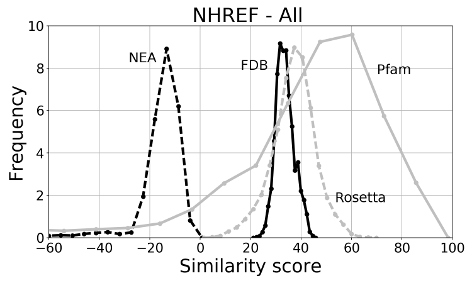
\includegraphics[width=8.4cm]{FDB/1G9O_simil_cut.png} &
       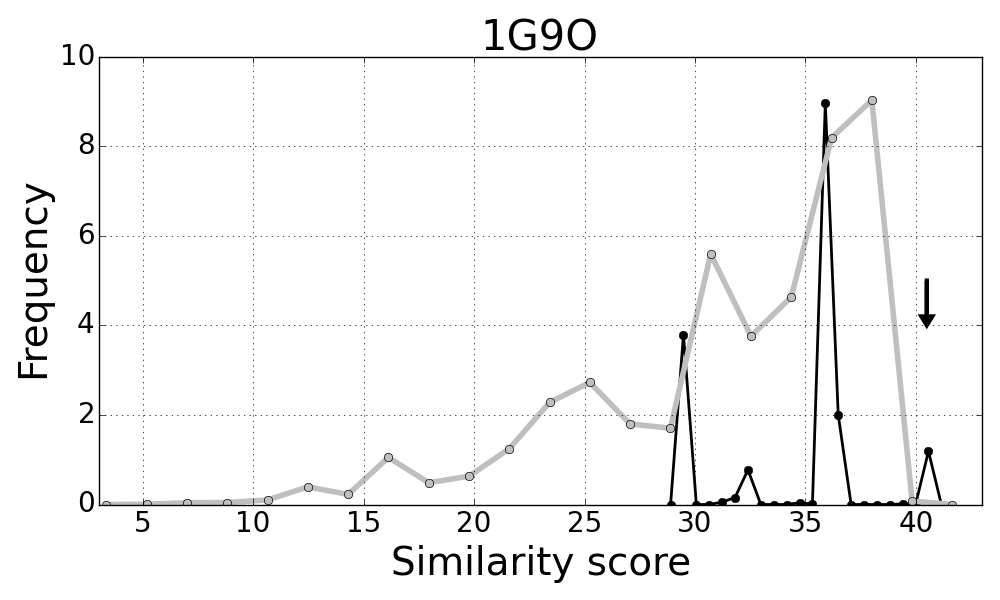
\includegraphics[width=8.4cm]{FDB/1G9O_simil_core.png} \\
       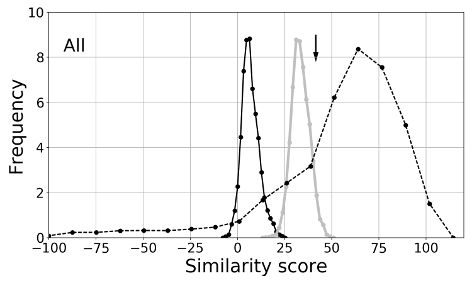
\includegraphics[width=8.4cm]{FDB/1R6J_simil_cut.png} &
       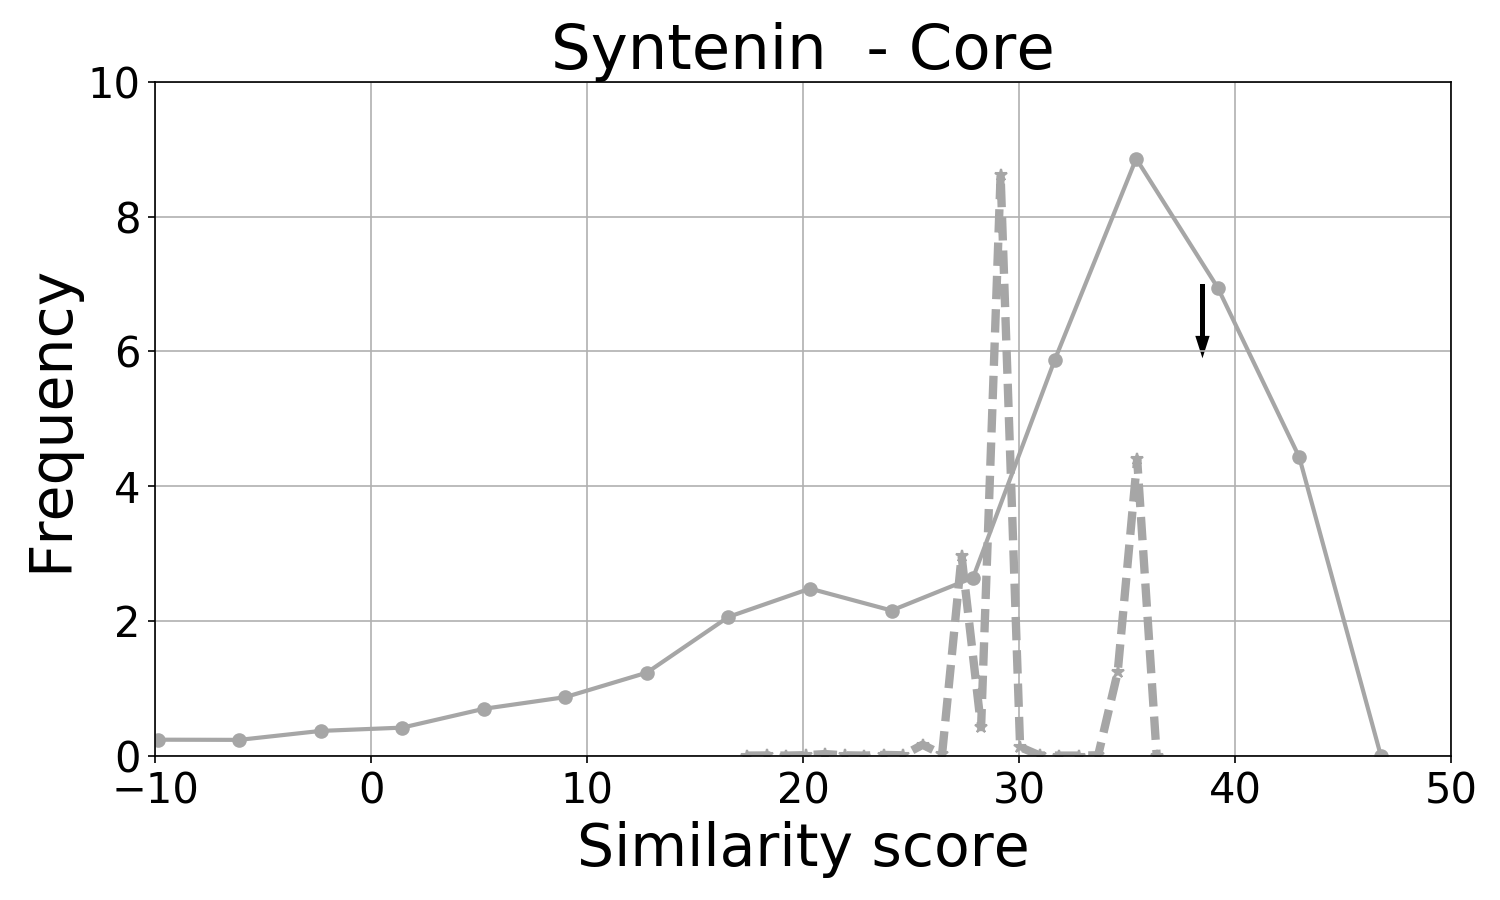
\includegraphics[width=8.4cm]{FDB/1R6J_simil_core.png} \\
       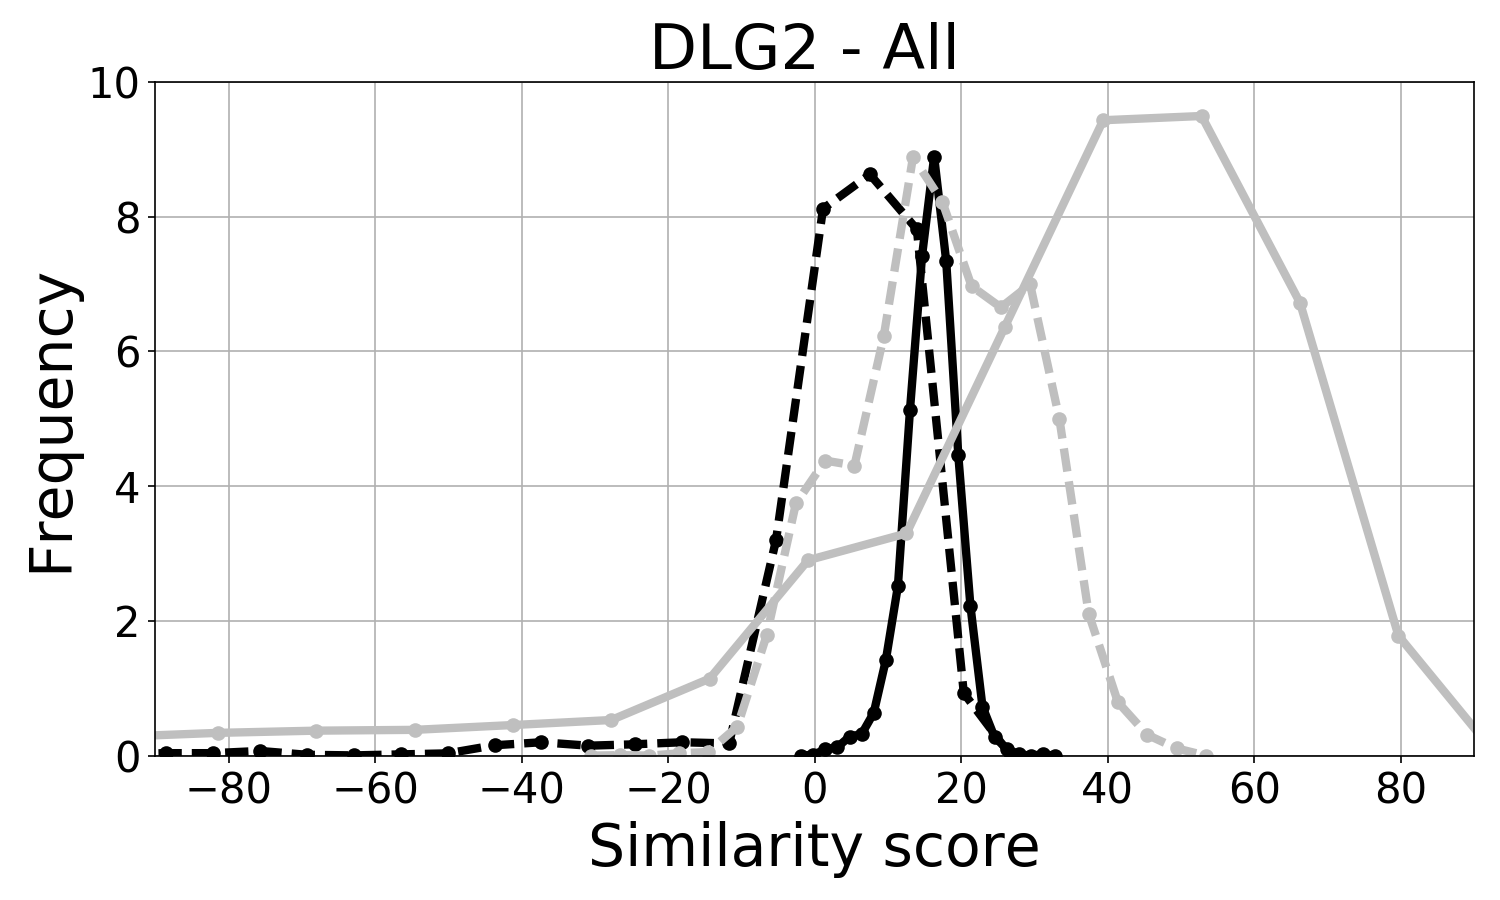
\includegraphics[width=8.4cm]{FDB/2BYG_simil_cut.png} &
       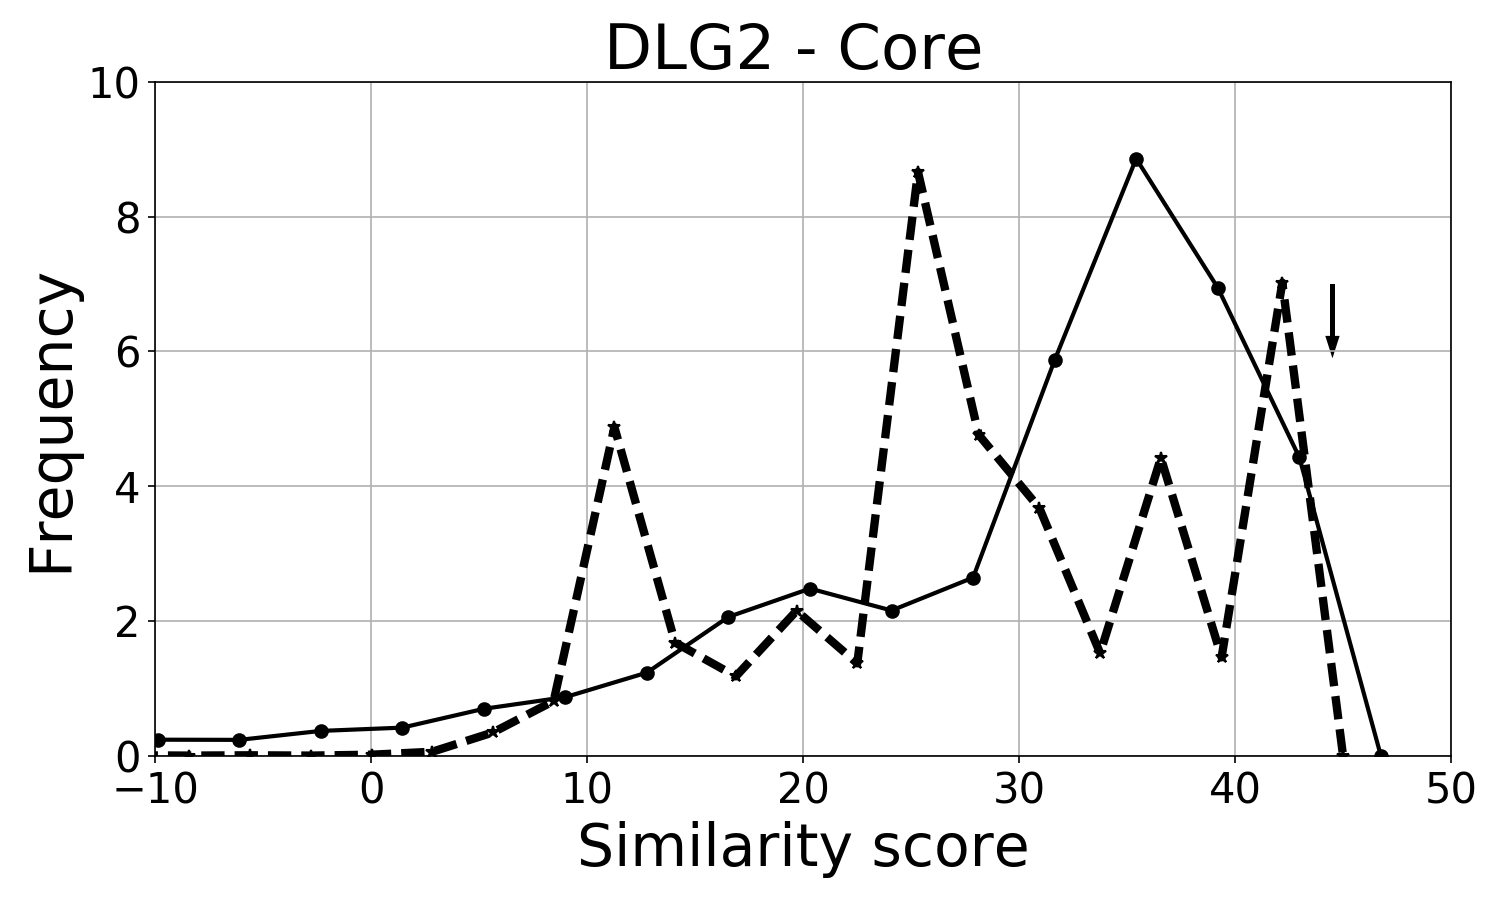
\includegraphics[width=8.4cm]{FDB/2BYG_simil_core.png} \\
     \end{tabular}
     \caption{Similarité des séquences Proteus (NEA et FDB),Rosetta , et des séquences de l'aligenment Pfam RP55, sur toutes les positions à gauche  et sur les positions du coeur à droite.}

     \label{graph:Simil_control_B}
   \end{figure}
    
\section{Application: Croissance du noyau hydrophobe}
Comme application de nos modèles optimisés, nous examinons la possibilité de conception du cœur hydrophobe des domaines PDZ. Chaque domaine PDZ est soumis à une simulation REMC avec une succession de fonctions énergétiques biaisées qui favorisent de plus en plus les résidus hydrophobes. La première simulation comprend un terme d'énergie de biais $\delta =0,4 kcal/mol$ (par position) qui pénalise les types d'acides aminés hydrophobes (I,L,M,V,A,W,F et Y). La dernière simulation comprend un terme d'énergie de biais $\delta = -0.4 kcal/mol$ (par position) qui favorise les types hydrophobes. Les valeurs d'énergie de biais intermédiaire $\delta =0,2 kcal/mol$ et $\delta = -0,2 kcal/mol$ sont également simulé. En diminuant progressivement la valeur du biais d'énergie $\delta$, nous "titrons" efficacement dans les résidus hydrophobes.

Les résultats pour Tiam1 sont présentés à la figure 7. À la plus grande valeur, $\delta$ le cœur hydrophobe de Tiam1 est "réduit" avec 10 positions d'acides aminés (sur 94) qui changent en un type polaire. Les positions modifiées se situent principalement sur le bord extérieur du noyau. A la valeur intermédiaire de $\delta$, le noyau hydrophobe ne compte plus que 4 changements es type polaire par rapport un cœur natif. À la valeur de $\delta$ la plus négative, le cœur hydrophobe devient plus grand, s'étendant vers les régions de surface , avec 14 positions polaires changées en type hydrophobe. Ainsi le nombre de positions modifiées est approximativement symétrique ( environ +/- 12 changements), reflétant le biais. Environ 2/3 des changements se produisent dans des éléments de structure secondaire. Dans l'ensemble, les propensions observées de chaque position à devenir polaire ou hydrophobe en présence d'un biais de pénalité petit ou grand d'énergie $\delta$ peuvent être considérées comme un indice de conception hydrophobe. Ici, 11 des 14 positions du cœur conservées (toute sauf les positions 884,898 et 903) sont restées hydrophobes même au plus haut niveau de biais polaire, avec 13 autres positions, indiquant que ces positions ont la plus grande propension à être hydrophobe. De plus, 14 positions ont changé de polaire à hydrophobe qu niveau de polarisation le plus élevé, indiquant que ces positions aussi ont une certaine propension a être hydrophobe. Les résultats pour Cask sont similaires, avec 11 positions changés en polaire au plus haut biais et 9 changés en hydrophobe au plus haut biais  hydrophobe.


    \begin{figure}[h]
      \centering
      \begin{tabular}{c}
        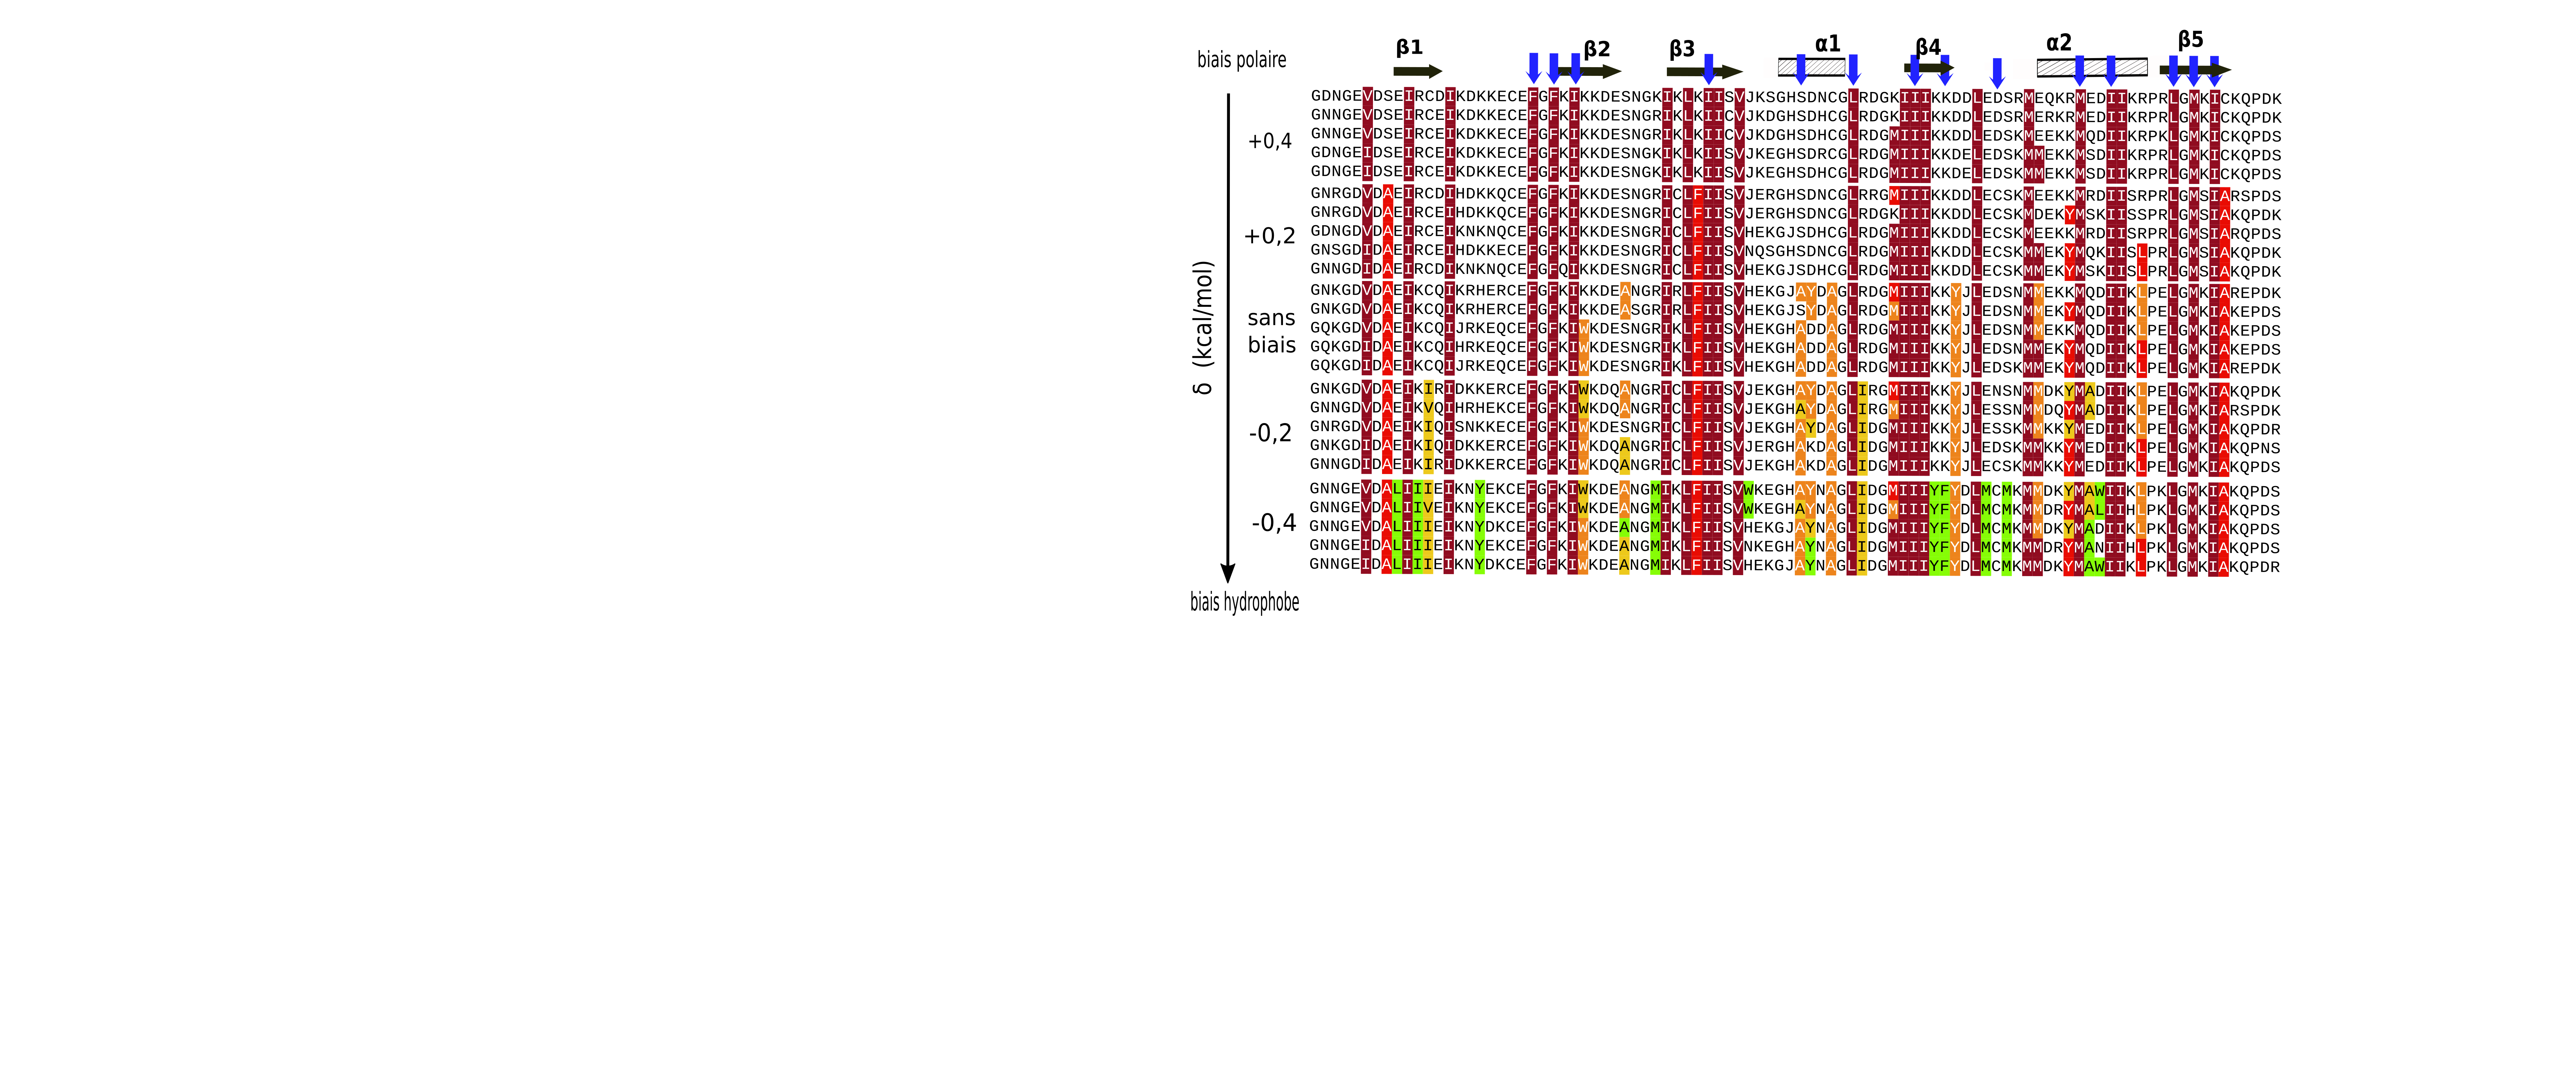
\includegraphics[width=14cm]{titration/alignTiam1.png} \\
      \end{tabular}

      \caption{\small Séquences Tiam1 obtenues avec un delta des énergies de références à -0.4,-0.2,0,0.2 et 0.4 et la struture native.Les hydrophobes pour des deltas de -0.4,-0.2,0,0.2 et 0.4 sont représentés par un dégradé allant du rouge foncé au vert clair, en passant par le jaune.}
      
      \label{titration_Tiam1}
    \end{figure}


    \begin{figure}[h]
      \centering
      \begin{tabular}{c}
        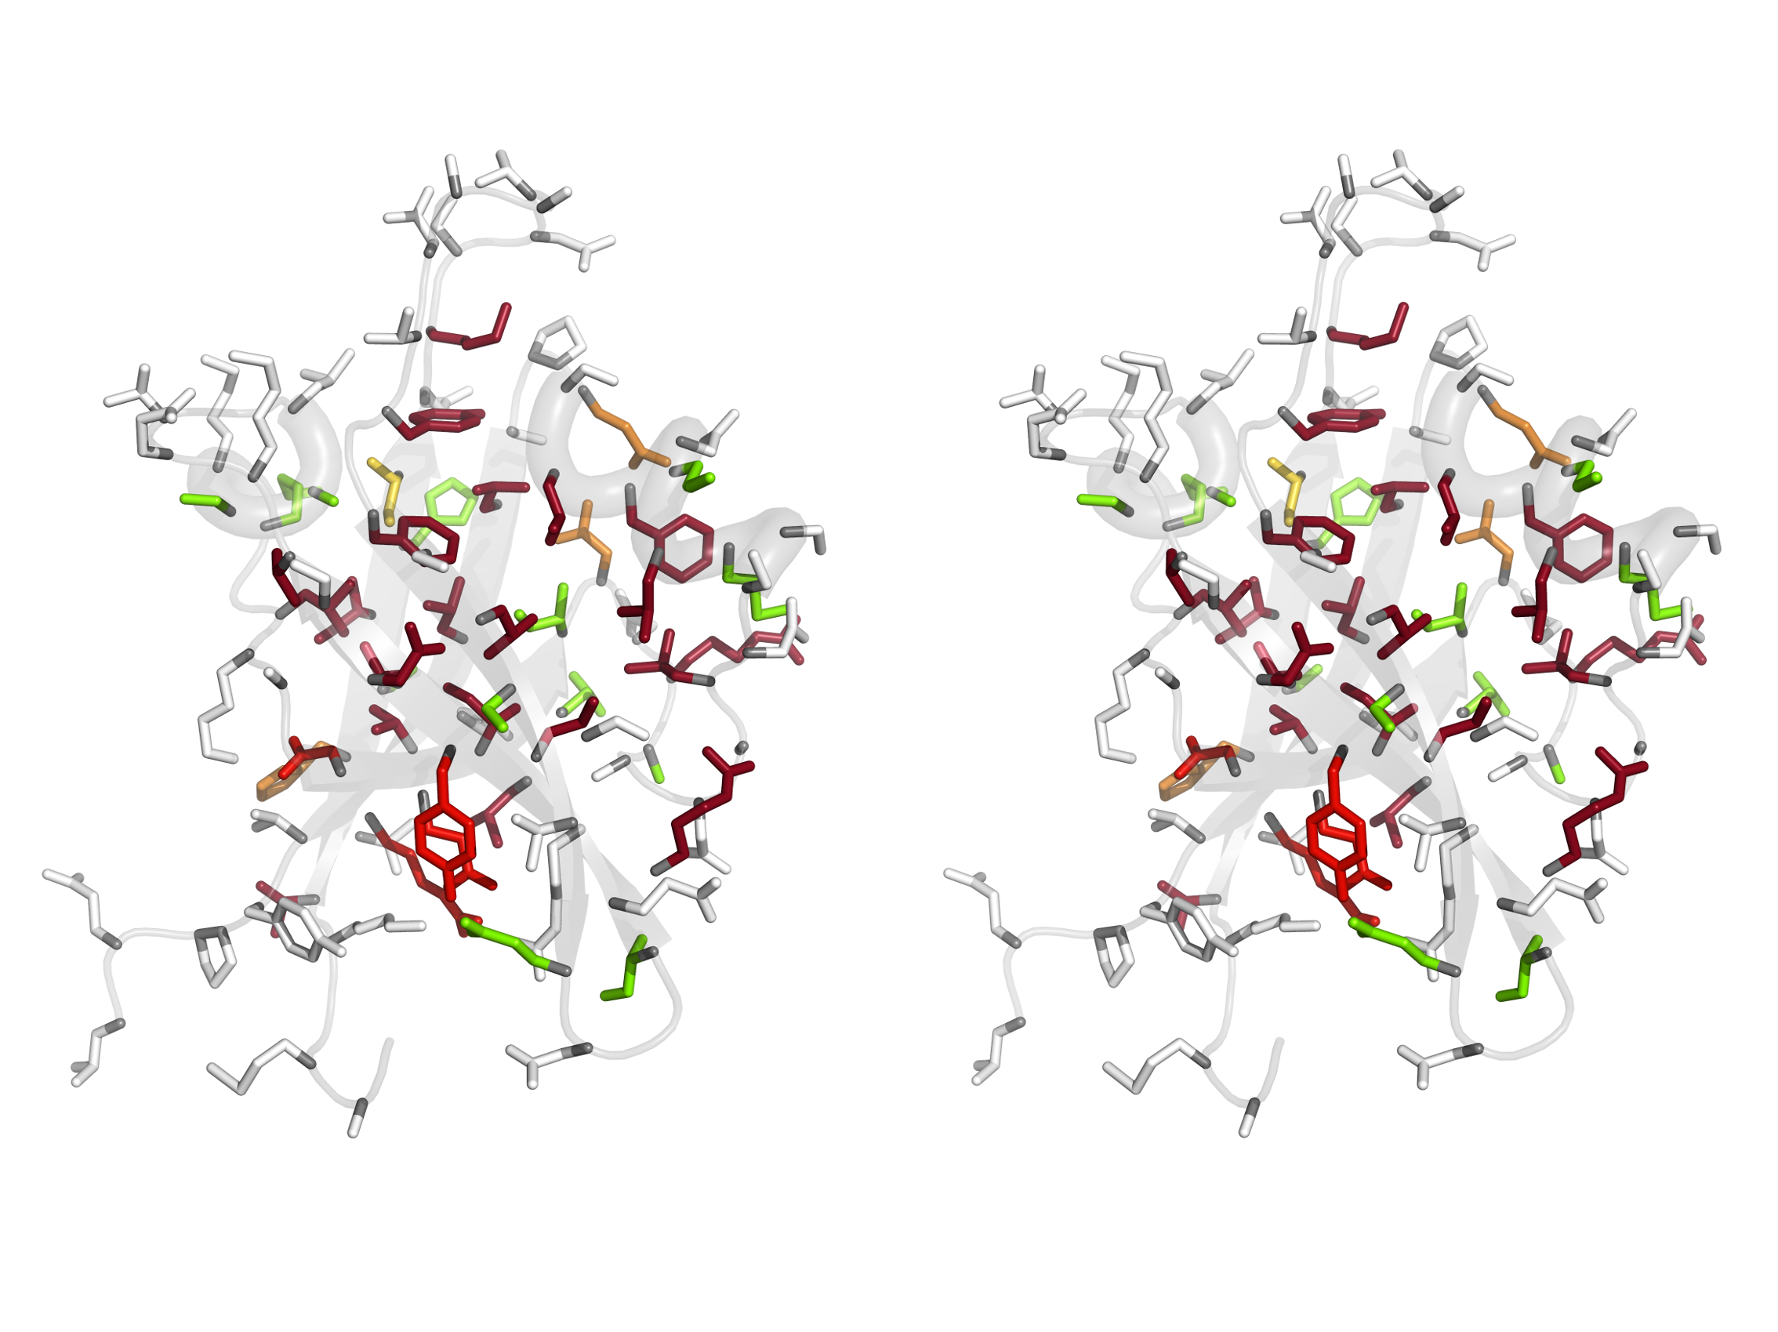
\includegraphics[width=15cm]{titration/structure_Tiam1.png} \\
      \end{tabular}

      \caption{\small Structure native Tiam1 avec les hydrophobes pour des deltas de -0.4,-0.2,0,0.2 et 0.4 sont représentés par un dégradé allant du rouge foncé au vert clair, en passant par le jaune.}
      
      \label{titration_Tiam1}
    \end{figure}

    

Nous calculons également un paramètre pour décrire le nombre de changements relatifs de type d'acide aminé par unité de l'énergie du biais. Ce  paramètre est défini comme le nombre $\delta N$ de positions de résidu  changées de non polaire à polaire, divisé par le produit de la variation $\delta E$ dans l'énergie de polarisation et le nombre moyen N de position non polaire à biais nul. Nous l'appelons la sensibilité hydrophobe $\psi_h$ . Pour le domaine PDZ Tiams1, ce calcul donne:
$\psi_h = \frac{1}{N} frac{\delta N}{\delta E} = 0,88$ changements par position et par kcal/mol. Pour Cask, la sensibilité hydrophobe  est  $\psi_h = 0,71$ changements par position et par kcal/mol.


\begin{figure}[!h]
  \centering
  \begin{tabular}{c}
    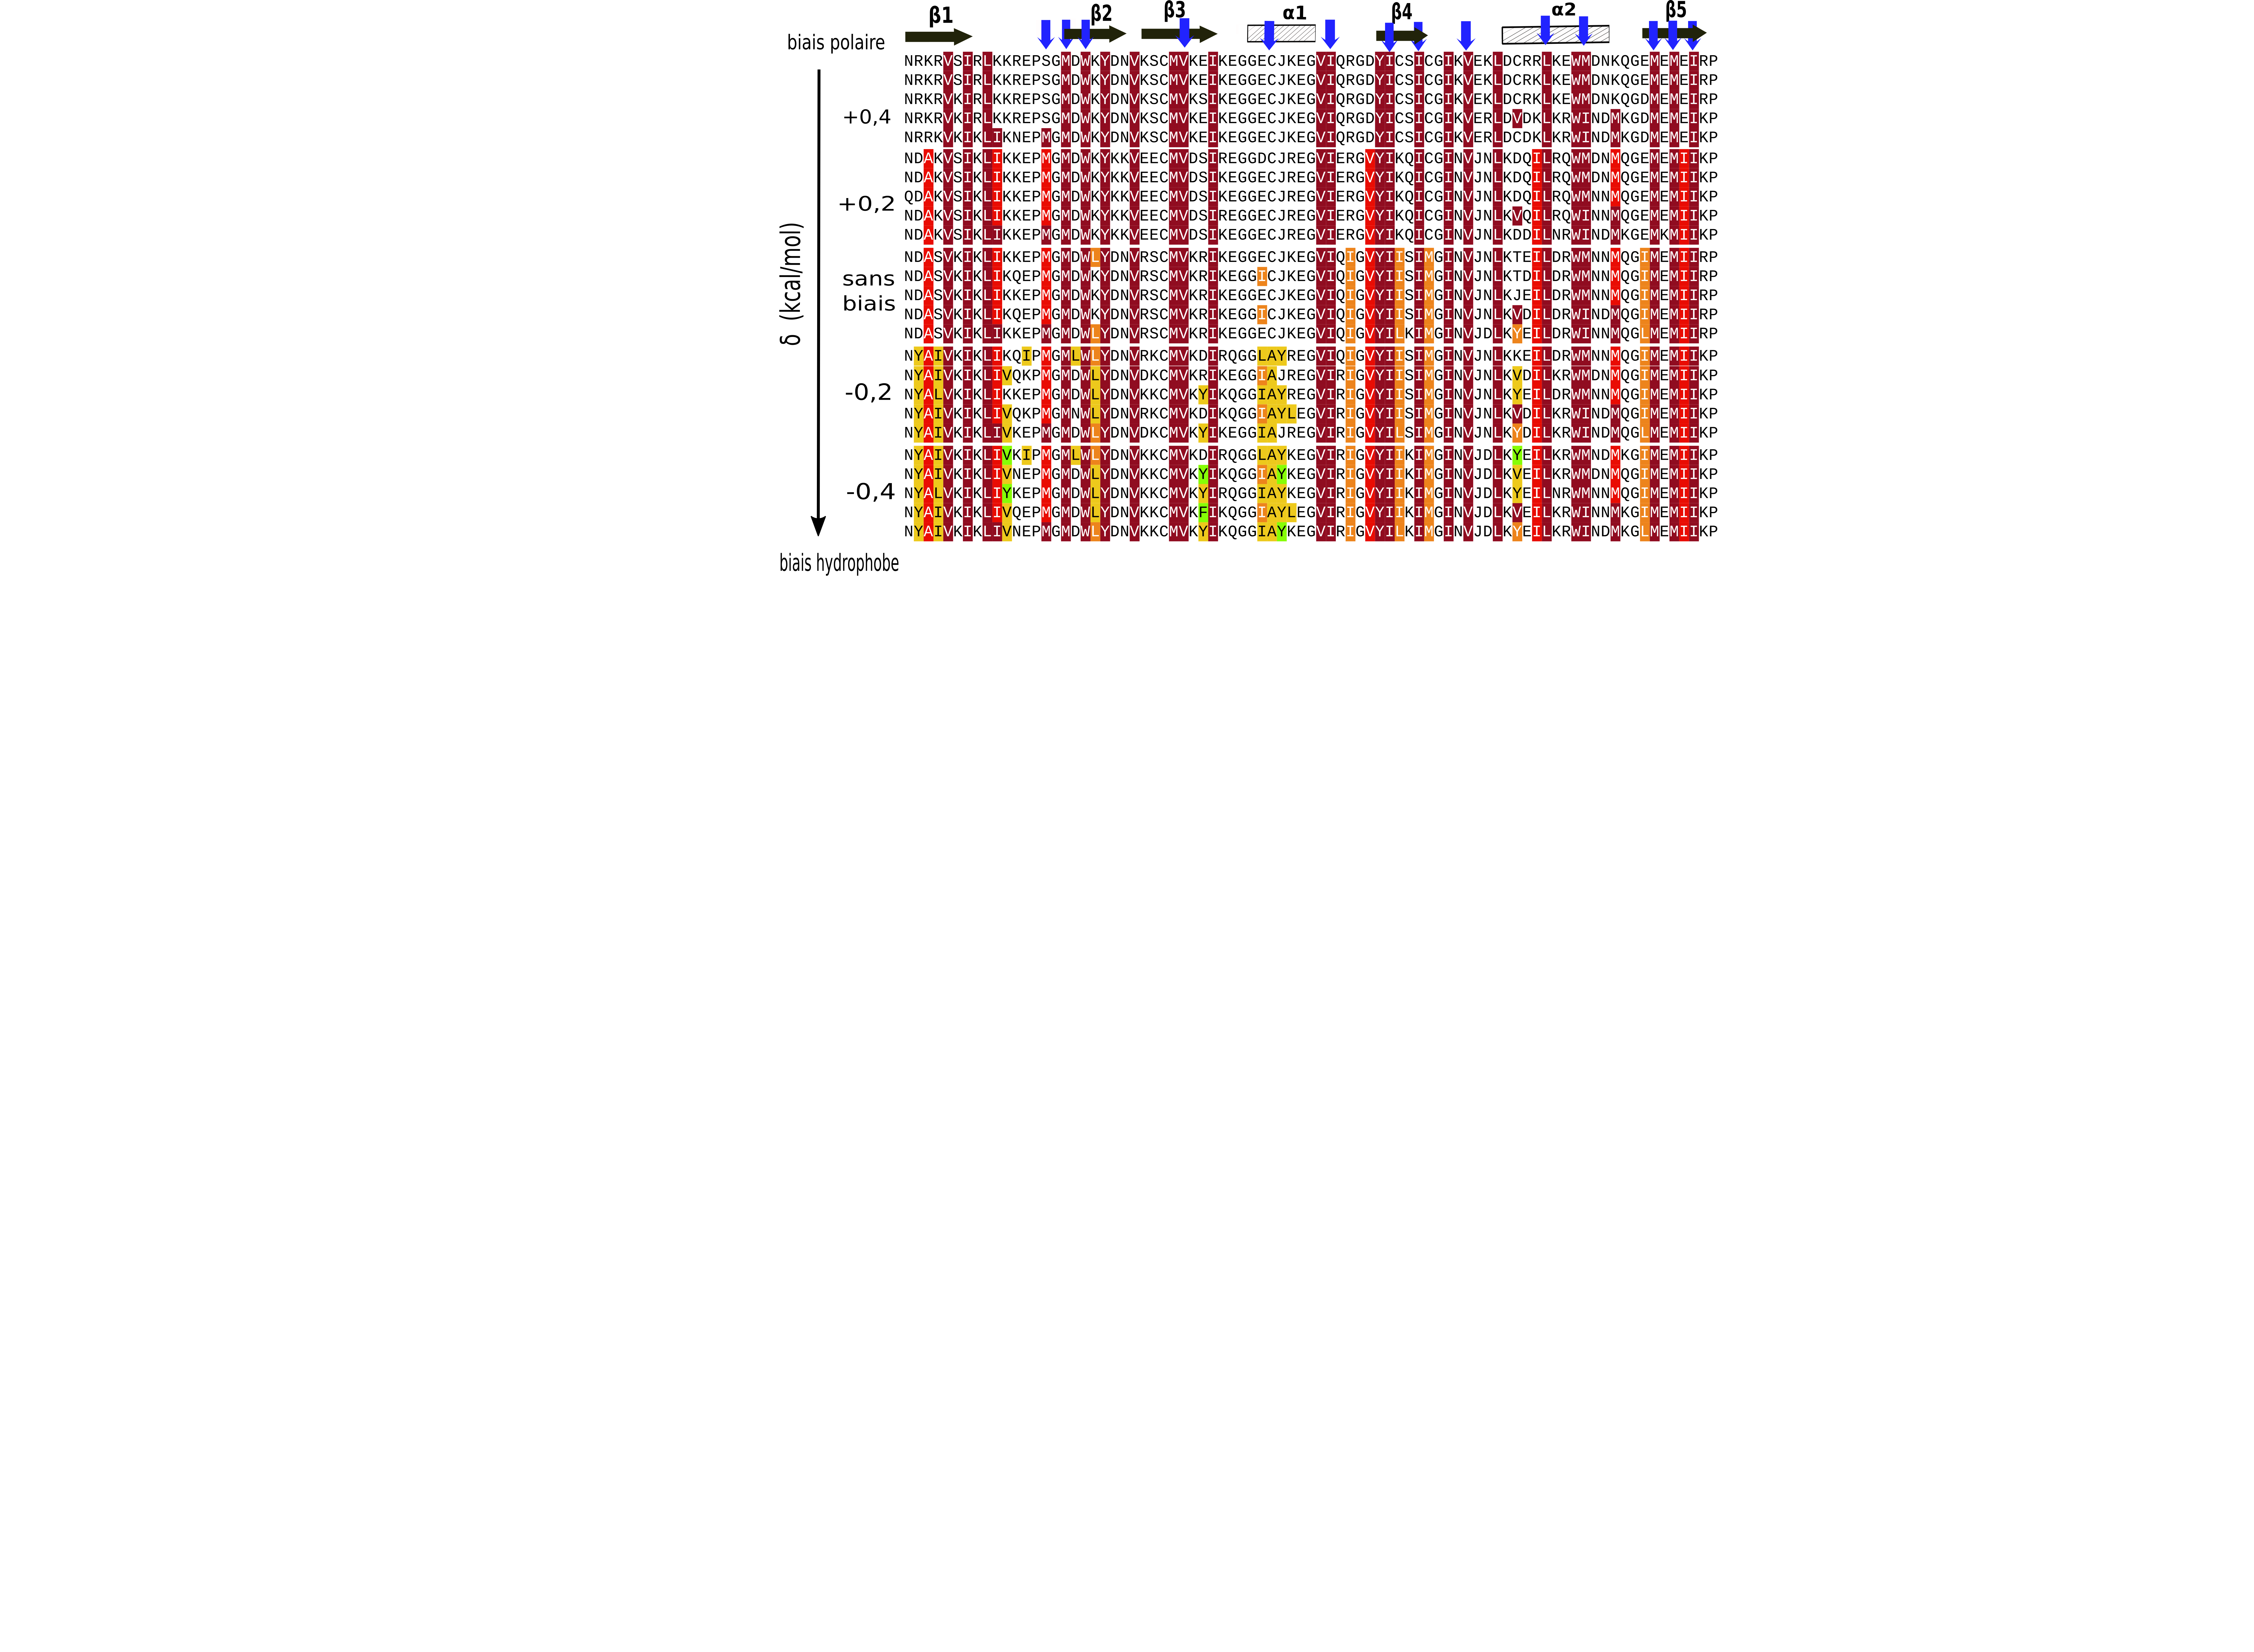
\includegraphics[width=16cm]{titration/alignCASK.png} \\
  \end{tabular}
  
  \caption{\small Séquences Cask obtenues avec un delta des énergies de références à -0.4,-0.2,0,0.2 et 0.4 et la struture native.Les hydrophobes pour des deltas de -0.4,-0.2,0,0.2 et 0.4 sont représentés par un dégradé allant du rouge foncé au vert clair, en passant par le jaune.}
  \label{result:PDZ_seed}
\end{figure}




\section{Conclusion}

\subsection{limites du modèle}

Nous paramétrons un modèle CPD simple pour la conception de domaine PDZ, adapté aux applications à conception de nombreuses séquences et mis en œuvre dans le logiciel Proteus. Pour la modélisation de l'état replié, nous utilisons un champ de force protéique de haute qualité. Nous avons testé deux ensembles de paramètres d'énergie de surface atomique $\sigma_i$ et deux modèles de solvant "GB généralisé", le modèle NEA et le FDB, avec une constante diélectrique $\epsilon_P = 8$  pour le NEA ,et $\epsilon_P = 4$ pour le FDB quantités  qui caractérisent  le modèle de solvant et sont les principaux paramètres empiriques dans la fonction d'énergie de l'état replié. Pour les chaînes latérales, nous utilisons une bibliothèque de rotamères simple et discrète et une petite minimisation de chaque paire pendant le calcul de la matrice d'énergie pour atténuer l'approximation de la discrétisation des rotamères. La fonction d'énergie et la description des rotamères ont été testées de manière approfondie et ont démontré de très bonnes performances pour les tests reconstruction de chaînes latérales \cite{Gaillard16} (comparable au programme populaire Scwrl4 (\cite{Krivov09}) ) et de bonnes performances pour sur un grand ensemble de constant acide/base de protéine \cite{Polydorides13} (supérieure au logiciel Rosetta (\cite{Kilambi12}), malgré un important réglage de paramètres ad hoc).

La représentation de l'état déplié utilise un modèle simple caractérisé par un ensemble de potentiels chimiques d'acide aminé empiriques ou énergies de référence. Ces énergies sont choisies par une procédure de maximisation de la probabilité, formulée ici, afin de reproduire la composition d'acides aminés d'homologues naturels soigneusement sélectionnés. L'état déplié utilisé ici est plus raffiné qu'auparavant, puisque des valeurs d'énergies de référence distinctes sont utilisées pour les positions d'acides aminés qui sont enfuis ou exposés à l'état replié.  

Cette méthode suppose qu'il existe une structure résiduelle à l'état déplié, où certaines positions sont plus enfuies que d'autres. En outre, cela doit rendre le paramétrage plus robuste et moins sensible à la taille et à la structure des homologues naturels utilisés pour définir les compositions d'acide aminé cibles, car les fréquences d'acide aminé des positions exposées et des régions enfouies sont calculées séparément. En principe, cela double le nombre d'énergie de référence à ajuster. Cependant, nous avons réduit ce nombre en introduisant des classes de similarité d''acide aminé, avec une énergie de référence ajustable par classe. Contrainte qui est levée en fin d'optimisation. Lors de l'optimisation d’ énergie de référence, nous effectuons, des calcules de séquences pour chaque protéine de notre jeu de test (à l'état apo) où une position sur deux  peut muter, soit la moitié des positions ( à l'exception de Gly et Pro), avec une simulation distincte pour chaque moitié. De cette façon, lors de l'optimisation des paramètres, une position mutable est toujours entourée d'un environnement  identique au type sauvage au moins sur les deux positions immédiatement voisines sur le squelette. Les calculs de conception des protéines s'appuient sur une méthode d'exploration Monte-Carlo avec échange de réplique, puissante et efficace, qui utilise plus d'un demi-miliard de pas par simulation et par réplique, et  produit des milliers de séquences dans une seule simulation. Les valeurs des énergies de référence sont optimisées avec deux choix différents du couple modèle de solvant constante diélectrique des protéines $\epsilon_p$. Les performances sont améliorées pour le modèle FDB.
Le modèle présente plusieurs limitations, dont la plupart se trouvent dans les implémentations et les applications du CPD. La première est l'utilisation de la stabilité des protéines comme seul critère de conception, sans prendre en compte explicitement la spécificité du pli \cite{Schmidt08,Simonson13}, la protection contre l'agrégation , ou des considérations fonctionnelles comme la liaison des ligands. Toutefois, nous notons que les tests superfamily n'ont pas entraînés de mauvaises affectations ( séquences perçues comme préférant un autre pli SCOP), donc en pratique, la spécification du pli est réalisée. La limitation supplémentaire est introduite  par l'utilisation d'un squelette protéique fixe lors du calcul de la matrice d'énergie. En fait, le squelette n'est pas vraiment fixe, certains mouvements sont autorisés, mais modélisés implicitement, à travers l'utilisation d'une constante diélectrique protéique supérieure à 1 ($\epsilon_p= 4$ ou 8) (78). Cette valeur diélectrique signifie que la structure protéique (y compris son squelette) est autorisée à se détendre ou à se réorganiser en réponse à une redistribution de charge associée à des mutations ou a un changement de rotamères de la chaîne latérale. Cependant, la réorganisation est modélisée non pas explicitement mais implicitement (78), et elle n'implique pas de mouvement des centres atomiques ou de leur sphère de Van der Waals associée. Ainsi, le squelette ne peut ni se réorganiser en réponse à une répulsion stérique produite par des mutations ou des changements de rotamères ni se déplacer pour remplir l'espace laissé vide par une mutation.  
L'utilisation d'un squelette fixe peut être en partie compensé en concevant plusieurs structures PDZ. Par exemple, la mise en commun des séquences calculées de Tiam1 et Cask a donnée une entropie moyenne de séquence comparable à celle de l'ensemble expérimental  Pfam, et nous a permis d'inventorier plus de séquences que les calculs avec un seul squelette. Notez qu'une nouvelle méthode pour la conception de protéine multi-backbone a récemment été développée dans Proteus, sur la base d'une méthode Monte-Carlo hybride qui préserve l'échantillonnage de la distribution de Boltzmann \cite{Druart17}. Cette méthode pourra être appliquée dans les prochaines études.
Une autre limitation de notre modèle est la nécessité, pour des résultats optimaux, de paramètres les énergies de référence spécifiquement pour un ensemble donné de protéines. Cette étape est bien automatisée et de façon très parallèle. Cependant, cela implique plusieurs choix qui sont partiellement arbitraires. Ceux-ci comprennent le choix d'un ensemble de domaines protéiques pour représenter la protéine ou la famille d'intérêt. Nous devons également choisir un seuil de similarité pour définir les homologues cibles à partir desquels sont calculées les compositions expérimentales d'acides aminés. Ici, nous avons choisi d'utiliser les homologues de chaque membre de la famille, de calculer leurs compositions, puis la moyenne sur les six familles. Cette méthode a correctement fonctionné, mais d'autres choix sont possibles et il faut travailler davantage pour pouvoir tirer des conclusions définitives sur ces choix.

Une autre limitation de notre modèle est l'approximation de  la position des chaînes latérales en rotamères discrets. qui nécessite une certaine adaptation de la fonction d'énergie pour éviter les affrontements stériques exagérés. La méthode utilisée ici est la méthode de minimisation de la paire de résidus décrite précédemment (26,76).

Une cinquième limitation est l'utilisation d'un modèle de solvatation additif par paire ( comme dans la plupart des modèles CPD). Plus précisément, l'environnement diélectrique de chaque paire de résidus est supposé ici être celui de la structure native (ce qu'on appelle "Approvisionnement environnemental natif" ou NEA 74,76). Cela conduit à une fonction énergétique qui a la forme d''une somme sur les paires de résidus et peut être précalculée et stockée dans une matrice énergétique, qui sert alors de table de consultations pendant les simulations Monte-Carlo. Malgré cette approximation, le modèle a donné de bons résultats pour un grand nombre d' indices acide/base de référence, un problème très sensible au traitement électrostatique \cite{Polydorides13}. Certaines de ces limitations sont supprimées dans le modèle FDB. En particulier, comme la fonction d'énergie est principalement basée sur la physique, elle a pu être améliorée par implémentations d'un calcul "GB" plus exact. Par ailleurs, il a été mis en place un modèle amélioré pour la solvatation hydrophobe (80), qui est plus rapide et plus précise que notre terme d''énergie de surface actuelle (article préparation).

\subsection{modèle de test et applications}

Les séquences calculées sont largement comparées aux séquences naturelles, à travers des tests de reconnaissance du pli, des calculs de similarité et des calculs d'entropie. Dans les simulations, nous concevons la totalité de la séquence de la protéine, de sirte que toutes les positions  ( à l'exception de Gly et Pro) peuvent muter librement, soumis seulement à un biais vers la composition moyenne expérimentale des acides aminés ( à travers les énergies de références). Malgré la quasi-absence de biais expérimentaux ou de contraintes, les séquences obtenues ont une forte similitude globale avec les séquences naturelles de Pfam, mesurée par les scores de similarité Blosum40. Les scores obtenus sont, pour l'essentiel, comparables aux scores de similarité entre les paires de séquences Pfam entre elles.  Ainsi, les séquences conçues avec Proteus ressemblent à des homologues naturels modérément éloignés. La similitude est très forte pour les résidus au cœur de la protéine, comme cela a été observé dans des études CPD précédentes (30,72). En revanche, pour les résidus à la surface de la protéine, les scores de similarité sont proches de zéro, le score obtenu si l'on tirait au hasard les acides aminés a ces positions. Notez que de nombreux résidus de surface sont impliqués dans des interactions fonctionnelles, comme les onze résidus de liaison aux peptides dans les domaines PDZ. Les résidus de surface sont également sélectionnés selon l'évolution pour éviter l'agrégation ou des adhésions indésirables. La plupart de ces contraintes fonctionnelles ne sont pas explicitement prises en compte dans  notre protocole de design (bien que la fonction d'énergie soit indirectement la solubilité des protéines). Malgré les scores de similarité limités pour les régions de surface, la reconnaissance de pli avec l'outil Superfamily  appliquée aux meilleurs modèles conçus est presque parfaite. Les tests de reconnaissance de plis antérieurs qui utilisaient une fonction d'énergie plus simple donnaient un taux de reconnaissance de pli inférieur, à environ 85\% (pour un ensemble de tests plus large et plus diversifié) et des similitudes inférieures (15,50).De toute évidence, l'utilisation combinée d'un champ de force protéique amélioré, du solvant "GB" et des énergies de référence spécifiques à la famille conduisent à des séquences calculées sont proche des séquences natives et sans doute meilleures.

Les séquences Proteus ont également été comparées aux séquences obtenues avec le logiciel Rosetta , qui a lui-même été testé de manière approfondie. Sur la Base des scores de similarité de Blosum (par rapport aux séquences naturelles dans Pfam) et des tests de reconnaissance du pli, les séquences Proteus et Rosetta semblent être de la même qualité. Cependant, Rosetta fait moins de mutations que Proteus; de sorte que les scores d'identité, par rapport à la protéine de type sauvage correspondante, sont environ 6\%  plus haut chez Rosetta. Ce qui veut dire que Proteus modifie environ 5 positions en plus , en moyenne, par domaine PDZ. Ce nombre peut facilement être réduit en ajoutant à la fonction d'énergie de Proteus un terme  d'énergie de biais explicite qui augmente avec le nombre de mutations l'éloignant de la séquence de type sauvage. 

Une autre possibilité pour tester nos séquences  est d'utiliser les simulations de dynamique moléculaire. Nicolas Panel a testé dix séquences Tiam1 calculées dans des simulations MD assez longues, dans la forme apo, en utilisant le même champ de force protéique que dans le modèle CPD (champ de force Amber) et un modèle d'eau explicite. Ces séquences 

   \begin{figure}[t]
     \scalebox{0.8}{
       \begin{tabular}{c}
         \includegraphics[width=18cm]{logos/core.png} \\
       \end{tabular}
     }
     \caption{Les seq_logo du coeur hydrophode PDZ}
\label{graph:corePDZ}
   \end{figure}

   \begin{figure}[t]
     \scalebox{0.8}{
       \begin{tabular}{c}
         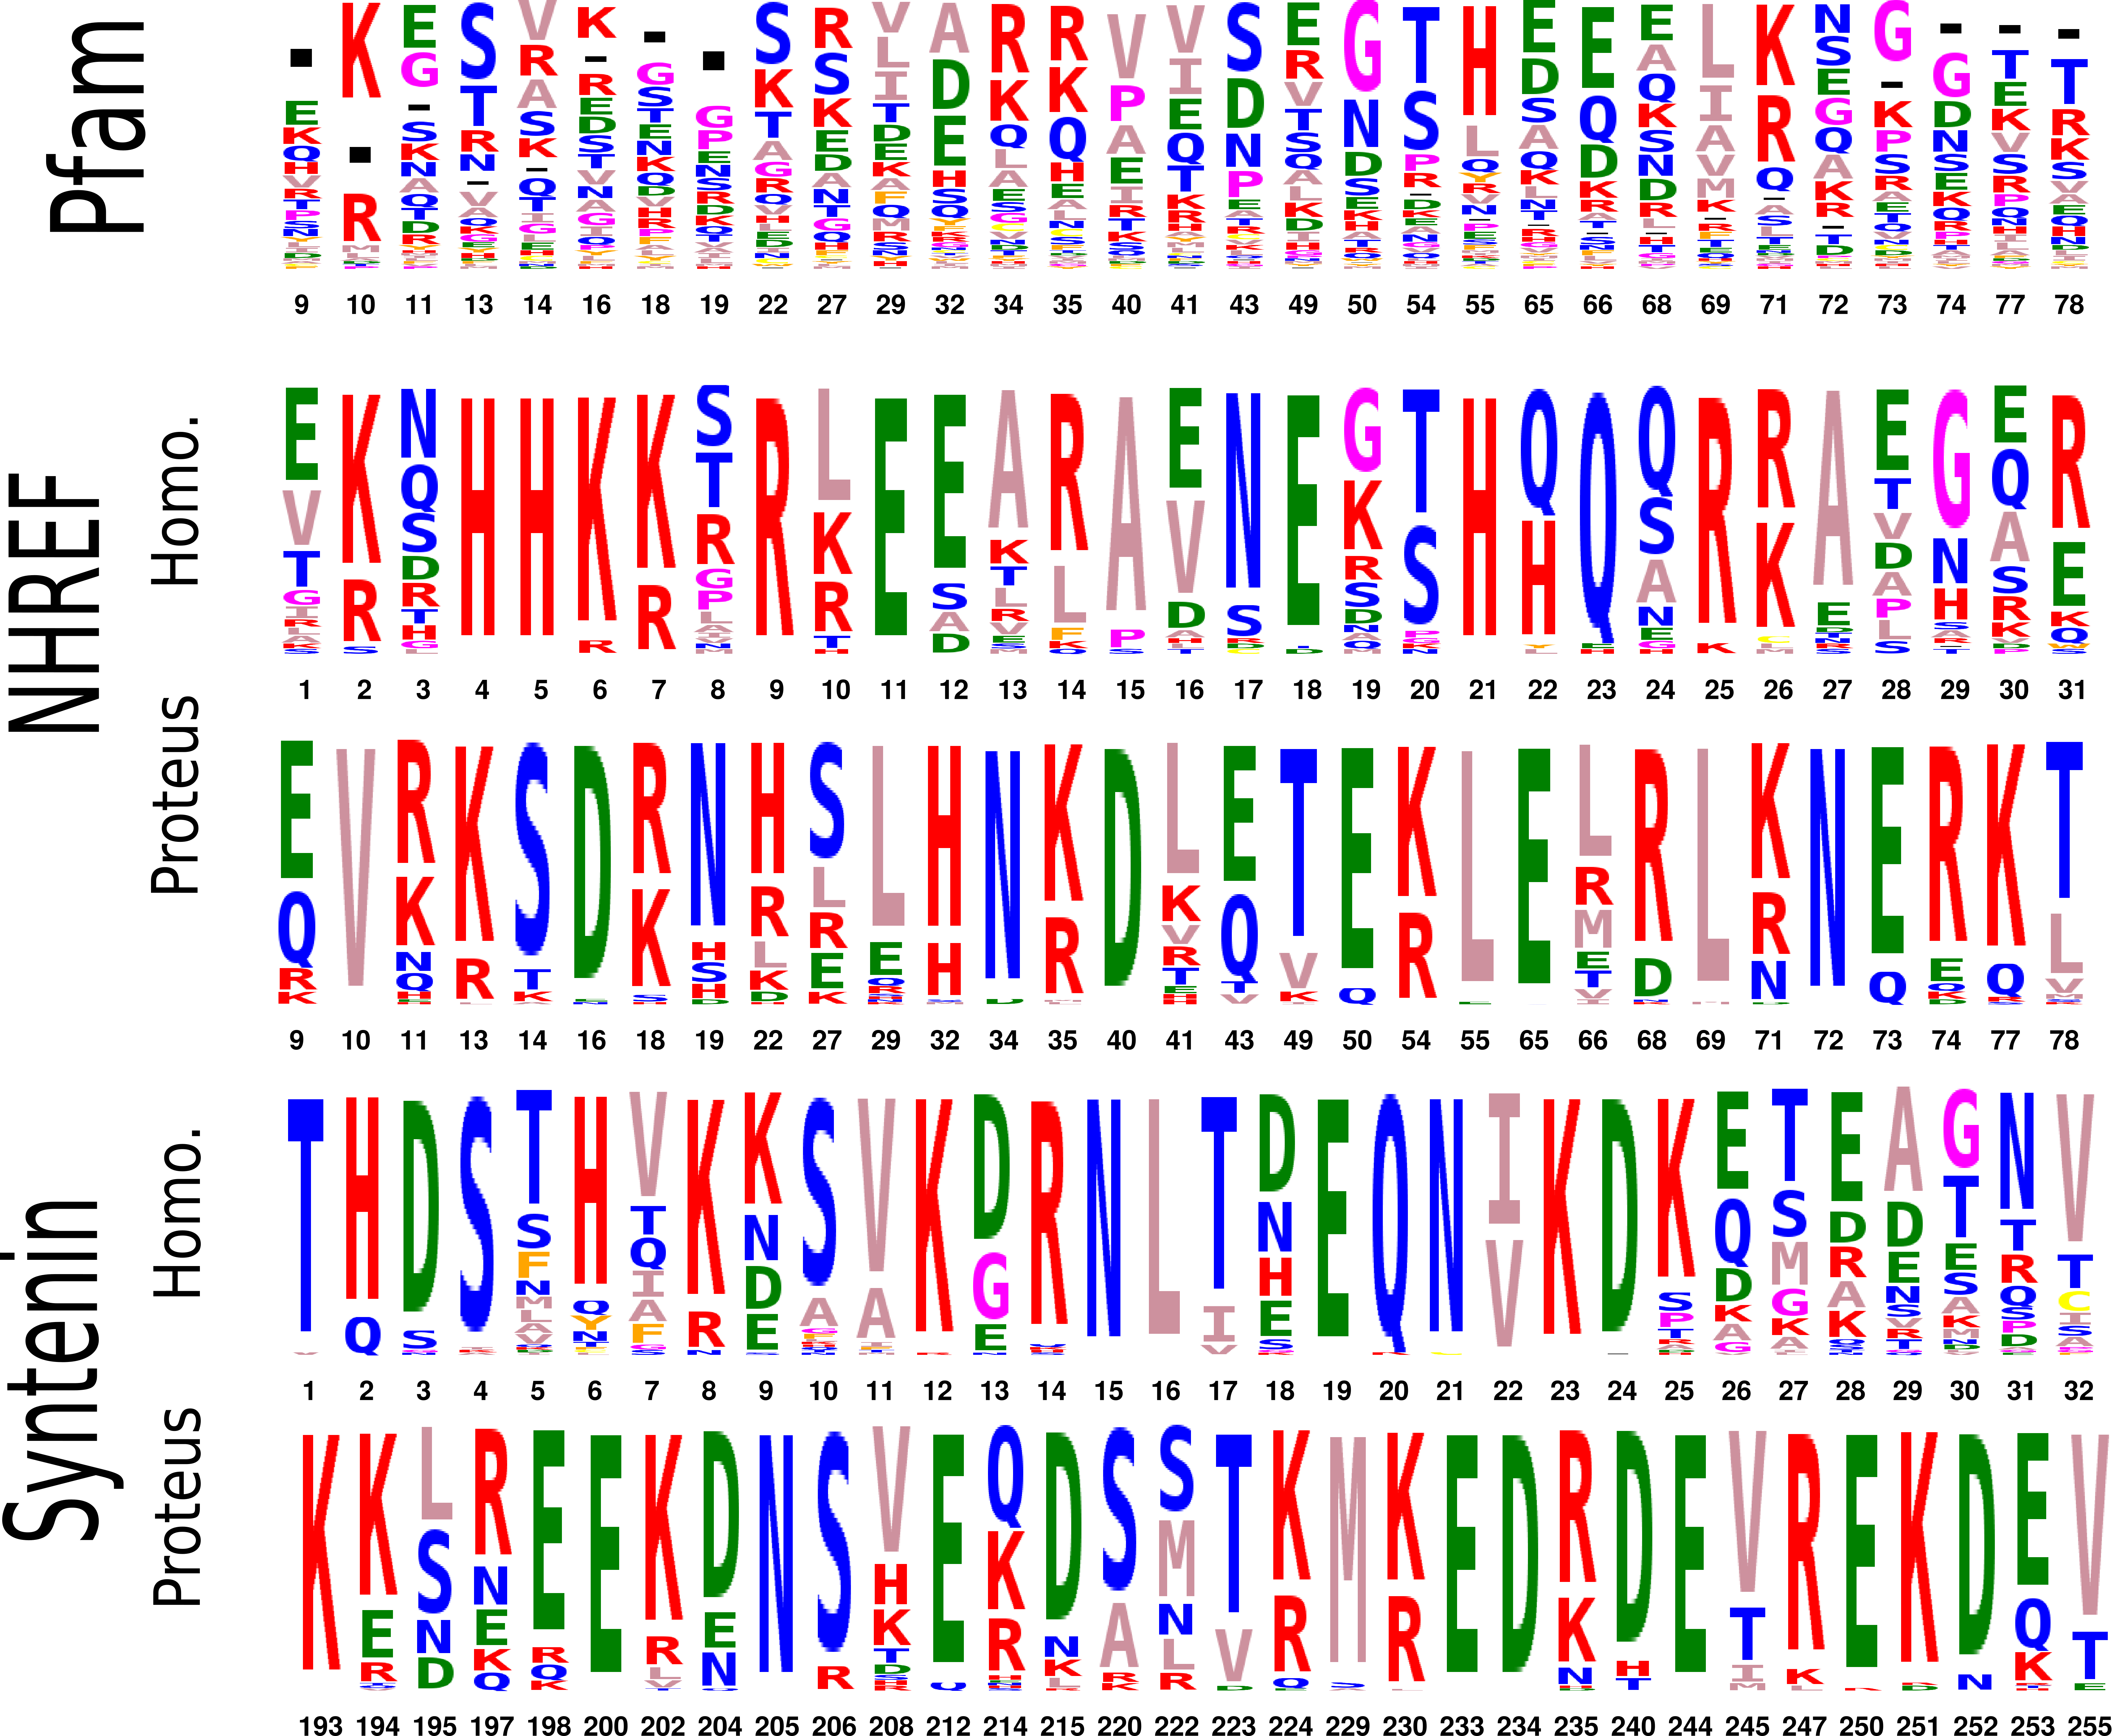
\includegraphics[width=18cm]{logos/exposed.png} \\
       \end{tabular}
     }
     \caption{Les seq_logo des positions exposées PDZ}
\label{graph:corePDZ}
   \end{figure}


   

%%% Local Variables:
%%% mode: latex
%%% TeX-master: "../these"
%%% End:
